\documentclass[../DoAn.tex]{subfiles}

\begin{document}
% Chương này có độ dài từ 9 đến 11 trang.

% Với phương pháp phân tích thiết kế hướng đối tượng, sinh viên sử dụng biểu đồ use case theo hướng dẫn của template này. Với các phương pháp khác, sinh viên trao đổi với giáo viên hướng dẫn để đổi tên và sắp xếp lại đề mục cho phù hợp. Ví dụ, thay vì sử dụng biểu đồ use case, sinh viên đi theo hướng tiếp cận Agile có thể dùng User Story.


% \textbf{Lưu ý}: Mỗi chương nên có thêm 1 đoạn mở đầu chương và kết thúc chương, mở đầu giới thiệu những nội dung sẽ trình bày trong chương, kết thúc tổng kết lại các nội dung đã trình bày


% START OF SECTION
\section{Khảo sát hiện trạng}
\label{section:2.1}
% Thông thường, khảo sát chi tiết về hiện trạng và yêu cầu của phần mềm sẽ được lấy từ ba nguồn chính, đó là (i) người dùng/khách hàng, (ii) các hệ thống đã có, (iii) và các ứng dụng tương tự.
% Sinh viên cần tiến hành phân tích, so sánh, đánh giá chi tiết ưu nhược điểm của các sản phẩm/nghiên cứu hiện có. Sinh viên có thể lập bảng so sánh nếu cần thiết. Kết hợp với khảo sát người dùng/khách hàng (nếu có), sinh viên nêu và mô tả sơ lược các tính năng phần mềm quan trọng cần phát triển.
Để lên ý tưởng, khảo sát nhu cầu, và tìm giải pháp cho bài toán, bằng cách áp dụng các phương pháp như phỏng vấn người dùng, tìm hiểu và nghiên cứu các hệ thống hiện có. Ta có thể chỉ ra được những cái thiếu sót, đặc điểm đặc biệt và đưa ra được các chức năng phù hợp.

\subsection{Phỏng vấn người dùng}
\label{section:2.1.1}
Các chủ cửa hàng nhỏ thường phải đối mặt với những thách thức trong việc quản lý hàng tồn kho và hóa đơn một cách hiệu quả và chính xác. Ví dụ trong các quầy thuốc, các hóa đơn, giấy ghi chép nhập xuất hàng theo thời gian trở lên càng nhiều. Hơn nữa, thống kê doanh thu trở lên lặp lại nhàm chán, tốn sức. Đặc biệt hơn, rất khó để biết chính xác được sản phẩm gì còn hay hết. Việc họ cần một ứng dụng điện thoại cầm tay để theo dõi lượng hàng tồn, và ghi chép lại doanh số bán hàng, hóa đơn sẽ giúp tiết kiệm thời gian và giảm thiểu tổn thất sai sót do việc thủ công bàn giấy.

\subsection{Khảo sát các hệ thống hiện có}
\label{section:2.1.2}
Trên thị trường hiện nay đã có ứng dụng giúp các doanh nghiệp quản lý tồn kho, hóa đơn và khách hàng như là KiotViet. Họ cung cấp đầy đủ chức năng nhưng đối tượng khách hàng nhắm đến quá rộng và ứng dụng của họ được thêm các chức năng mà các cửa hàng nhỏ hầu như không cần thiết.
\begin{itemize}
    \item \textbf{Quản lý và bán hàng}: Họ tách ra làm riêng 2 ứng dụng riêng lẻ khiến việc đổi ứng dụng để sử dụng khiến thêm thao tác thừa tốn thời gian.
    \item \textbf{Quảng cáo tiện ích}: Ứng dụng của họ hay có các quảng cáo về các dịch vụ tiện ích khác, lấy đi nhiều khoảng trống trên màn hình, gây khó chịu.
    \item \textbf{Chức năng sàn thương mại điện tử}: Họ cung cấp chức năng bán hàng trực tuyến, nhưng đối tượng khách hàng của họ là các doanh nghiệp lớn, không phù hợp với các cửa hàng nhỏ.
    \item \textbf{Dịch vụ theo tháng}: Để sử dụng ứng dụng, các cửa hàng phải bỏ ra một khoản tiền hàng tháng để có thể sử dụng và bị giới hạn chức năng, giới hạn số tài khoản người dùng theo gói đăng kí.
    \item \textbf{Dữ liệu không hoàn toàn kiểm soát}: Các dữ liệu khách hàng, hàng hóa đều nằm trên hệ thống của họ, khiến việc nếu các chủ cửa hàng muốn hoàn toàn nắm giữ dữ liệu và trích xuất ra các phần mềm khác bị khó khăn, phụ thuộc.
\end{itemize}
\vfill
\break


\subsection{Mục tiêu và phạm vi của đề tài}
\label{section:2.1.3}
Hệ thống đề xuất sẽ giải quyết các vấn đề như trên và đáp ứng được chính xác đối tượng khách hàng mà đề tài đề ra. Hệ thống sẽ được xây dựng với các mục tiêu chính như sau:
\begin{itemize}
    \item \textbf{Giao diện đơn giản}: Loại bỏ các chức năng không cần thiết, tập trung vào các chức năng chính, giúp người dùng dễ dàng sử dụng cho dù họ không có nhiều kinh nghiệm về công nghệ.
    \item \textbf{Hỗ trợ đa nền tảng}: Hệ thống được sử dụng bằng ứng dụng điện thoại chạy được trên Android, iOS.
    \item \textbf{Self-hosting}: Hệ thống được cài đặt trên máy chủ của người dùng, giúp người dùng hoàn toàn nắm giữ dữ liệu và có thể trích xuất ra các phần mềm khác. Ngoài ra, hệ thống cũng có thể được cài đặt trên các dịch vụ đám mây như AWS, Google Cloud, Azure, ... để giảm thiểu chi phí cho người dùng mà không bị giới hạn chức năng.
    \item \textbf{Lưu trữ đám mây}: Dữ liệu được lưu trữ trên đám mây, giúp người dùng có thể truy cập từ bất cứ đâu, bất cứ khi nào và tránh mất dữ liệu khi thiết bị bị hỏng.
    \item \textbf{Bảo mật dữ liệu}: Dữ liệu hoàn toàn được nằm trong máy chủ người dùng, hệ thống sẽ không lưu trữ bất cứ dữ liệu nào trên máy chủ của nhà phát triển.
    \item \textbf{Tính mở rộng}: Hệ thống có thể được thiết kế để hỗ trợ thêm các chức năng mới tùy theo nhu cầu của người dùng.
\end{itemize}
\break
% END OF SECTION

% START OF SECTION
\section{Tổng quan chức năng}
\label{section:general-function}
% Phần \ref{section:2.2} này có nhiệm vụ tóm tắt các chức năng của phần mềm. Trong phần này, sinh viên lưu ý chỉ mô tả chức năng mức cao (tổng quan) mà không đặc tả chi tiết cho từng chức năng. Đặc tả chi tiết được trình bày trong phần \ref{section:2.3}.


\subsection{Biểu đồ use case tổng quát}
\label{subsection:uc-general}
% Sinh viên vẽ biểu đồ use case tổng quan và giải thích các tác nhân tham gia là gì, nêu vai trò của từng tác nhân, và mô tả ngắn gọn các use case chính.
Hệ thống bao gồm các tác nhân được liệt kệ trong hình \ref{fig:uc-general}: Quản trị viên, Nhân viên, Quản lý. Phần lớn các use case đều xoay quanh các tác nhân Nhân viên và Quản lý. Quản trị viên chỉ có vai trò quản lý tài khoản người dùng, phân quyền truy cập hệ thống. Hệ thống gồm các use case tương ứng với từng thực thể chính: Sản phẩm (\ref{subsection:uc-product}), Phiếu nhập kho (\ref{subsection:uc-importreport}), xuất kho (\ref{subsection:uc-exportreport}), kiểm kho (\ref{subsection:uc-auditreport}), Hóa đơn (\ref{subsection:uc-invoice}), Khách hàng (\ref{subsection:uc-client}), Thông tin người dùng (\ref{subsection:uc-user}).

\begin{figure}[H]
    \centering
    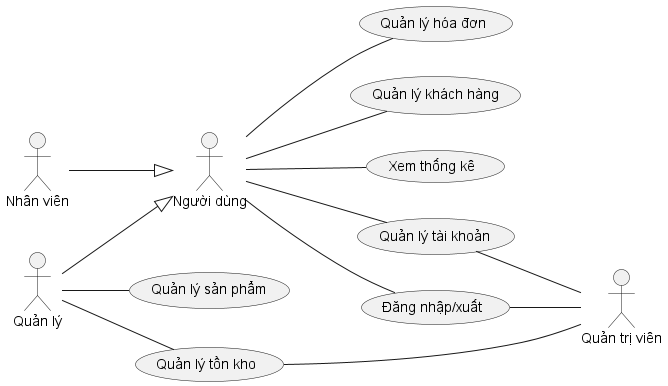
\includegraphics[width=0.75\textwidth]{Hinhve/usecases/General}
    \caption{Biểu đồ use case tổng quát}
    \label{fig:uc-general}
\end{figure}
\break


\subsection{Biểu đồ use case phân rã Xác thực người dùng}
\label{subsection:uc-authentication}
% Với mỗi use case mức cao trong biểu đồ use case tổng quan, sinh viên tạo một mục riêng như mục \ref{subsection:2.2.2} và tiến hành phân rã use case đó. Lưu ý tên use case cần phân rã trong biểu đồ use case tổng quan phải khớp với tên đề mục.
% Trong mỗi mục như vậy, sinh viên vẽ và giải thích ngắn gọn các use case phân rã.
Như được mô tả trong hình \ref{fig:uc-authentication}. Use case này bao gồm hai use case con: Đăng nhập và Đăng xuất. Đăng nhập được sử dụng khi người dùng muốn đăng nhập vào hệ thống. Đăng xuất được sử dụng khi người dùng muốn đăng xuất khỏi hệ thống.

\begin{figure}[H]
    \centering
    \includegraphics[width=0.7\textwidth]{Hinhve/usecases/Authentication}
    \caption{Biểu đồ use case phân rã Xác thực người dùng}
    \label{fig:uc-authentication}
\end{figure}


\subsection{Biểu đồ use case phân rã Sản phẩm}
\label{subsection:uc-product}
Như được mô tả trong hình \ref{fig:uc-product}. Use case này bao gồm các use case con: Lọc và xem sản phẩm, Quản lý sản phẩm, Tìm kiếm sản phẩm. Lọc và xem sản phẩm được sử dụng khi người dùng muốn lọc và xem thông tin sản phẩm. Quản lý sản phẩm được sử dụng khi người dùng muốn thêm, sửa, xóa sản phẩm. Tìm kiếm sản phẩm được sử dụng khi người dùng muốn tìm kiếm sản phẩm để thêm vào đơn từ.

\begin{figure}[H]
    \centering
    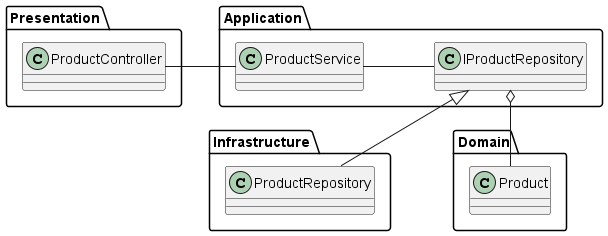
\includegraphics[width=0.9\textwidth]{Hinhve/usecases/Product}
    \caption{Biểu đồ use case phân rã Sản phẩm}
    \label{fig:uc-product}
\end{figure}


\subsection{Biểu đồ use case phân rã Nhập kho}
\label{subsection:uc-importreport}
Như được mô tả trong hình \ref{fig:uc-importreport}. Use case này bao gồm các use case con: Lọc và xem phiếu nhập kho, Quản lý phiếu nhập kho. Lọc và xem phiếu nhập kho được sử dụng khi người dùng muốn lọc và xem thông tin phiếu nhập kho. Quản lý phiếu nhập kho được sử dụng khi người dùng muốn thêm, hủy, xóa phiếu nhập kho.

\begin{figure}[H]
    \centering
    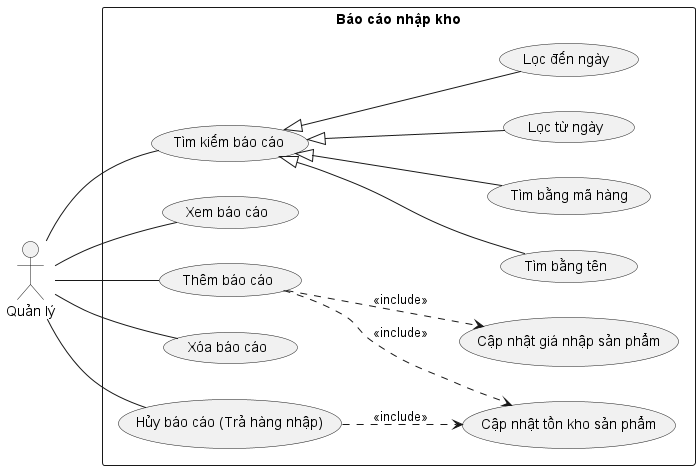
\includegraphics[width=0.8\textwidth]{Hinhve/usecases/ImportReport}
    \caption{Biểu đồ use case phân rã Nhập kho}
    \label{fig:uc-importreport}
\end{figure}


\subsection{Biểu đồ use case phân rã Xuất kho}
\label{subsection:uc-exportreport}
Như được mô tả trong hình \ref{fig:uc-exportreport}. Use case này bao gồm các use case con: Lọc và xem phiếu xuất kho, Quản lý phiếu xuất kho. Lọc và xem phiếu xuất kho được sử dụng khi người dùng muốn lọc và xem thông tin phiếu xuất kho. Quản lý phiếu xuất kho được sử dụng khi người dùng muốn thêm, hủy, xóa phiếu xuất kho.

\begin{figure}[H]
    \centering
    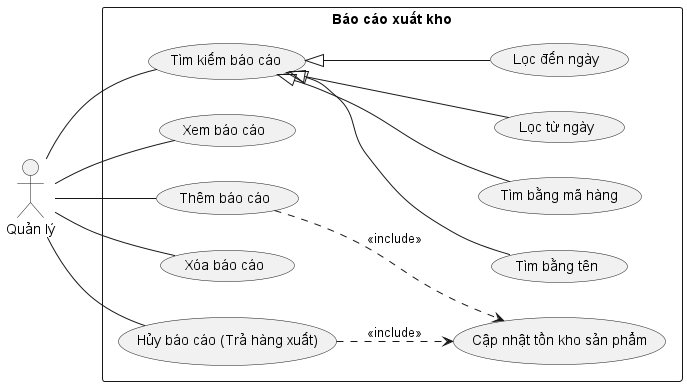
\includegraphics[width=0.8\textwidth]{Hinhve/usecases/ExportReport}
    \caption{Biểu đồ use case phân rã Xuất kho}
    \label{fig:uc-exportreport}
\end{figure}


\subsection{Biểu đồ use case phân rã Kiểm kho}
\label{subsection:uc-auditreport}
Như được mô tả trong hình \ref{fig:uc-auditreport}. Use case này bao gồm các use case con: Lọc và xem phiếu kiểm kho, Quản lý phiếu kiểm kho. Lọc và xem phiếu kiểm kho được sử dụng khi người dùng muốn lọc và xem thông tin phiếu kiểm kho. Quản lý phiếu kiểm kho được sử dụng khi người dùng muốn thêm, xóa phiếu kiểm kho.

\begin{figure}[H]
    \centering
    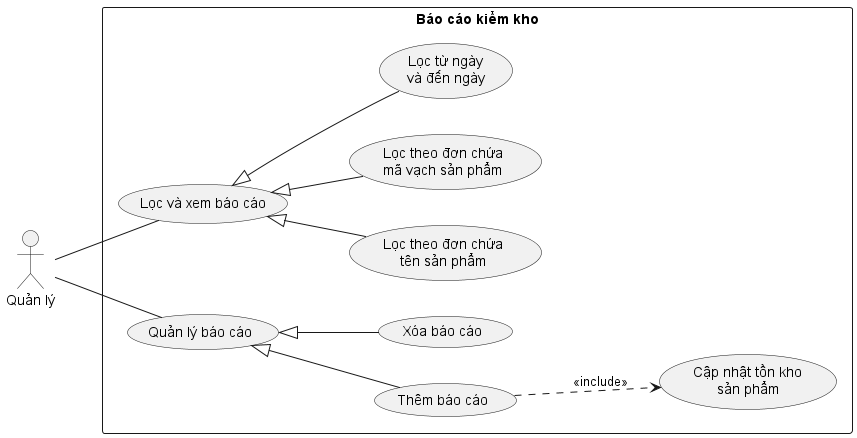
\includegraphics[width=0.9\textwidth]{Hinhve/usecases/AuditReport}
    \caption{Biểu đồ use case phân rã Kiểm kho}
    \label{fig:uc-auditreport}
\end{figure}


\subsection{Biểu đồ use case phân rã Khách hàng}
\label{subsection:uc-client}
Như được mô tả trong hình \ref{fig:uc-client}. Use case này bao gồm các use case con: Lọc và xem khách hàng, Quản lý khách hàng, Tìm kiếm khách hàng. Lọc và xem khách hàng được sử dụng khi người dùng muốn lọc và xem thông tin khách hàng. Quản lý khách hàng được sử dụng khi người dùng muốn thêm, sửa, xóa khách hàng. Tìm kiếm khách hàng được sử dụng khi người dùng muốn tìm kiếm khách hàng để thêm vào hóa đơn.

\begin{figure}[H]
    \centering
    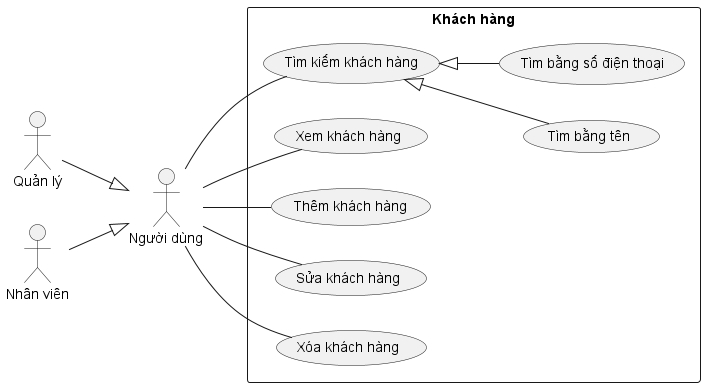
\includegraphics[width=0.7\textwidth]{Hinhve/usecases/Client}
    \caption{Biểu đồ use case phân rã Khách hàng}
    \label{fig:uc-client}
\end{figure}


\subsection{Biểu đồ use case phân rã Hóa đơn}
\label{subsection:uc-invoice}
Như được mô tả trong hình \ref{fig:uc-invoice}. Use case này bao gồm các use case con: Lọc và xem hóa đơn, Quản lý hóa đơn. Lọc và xem hóa đơn được sử dụng khi người dùng muốn lọc và xem thông tin hóa đơn. Quản lý hóa đơn được sử dụng khi người dùng muốn thêm, xóa hóa đơn.

\begin{figure}[H]
    \centering
    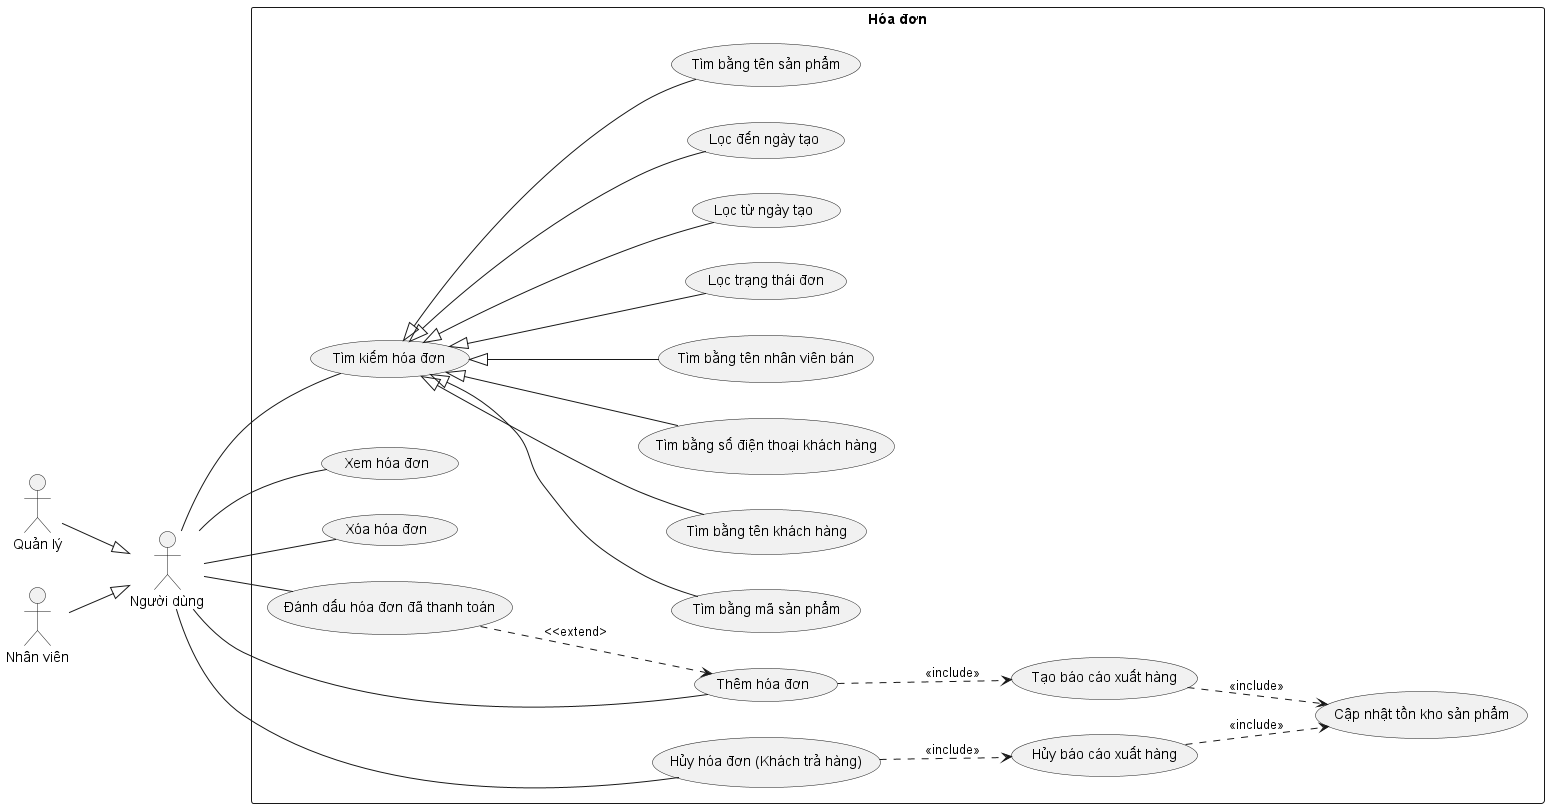
\includegraphics[width=\textwidth]{Hinhve/usecases/Invoice}
    \caption{Biểu đồ use case phân rã Hóa đơn}
    \label{fig:uc-invoice}
\end{figure}
\break


\subsection{Biểu đồ use case phân rã Thông tin người dùng}
\label{subsection:uc-user}
Như được mô tả trong hình \ref{fig:uc-user}. Use case này bao gồm các use case con: Quản lý thông tin người dùng, Quản lý thông tin cá nhân. Quản lý thông tin người dùng được sử dụng khi quản trị viên muốn thêm, sửa, xóa truy cập của người dùng hệ thống. Quản lý thông tin cá nhân được sử dụng khi người dùng muốn thay đổi thông tin cá nhân của mình.

\begin{figure}[H]
    \centering
    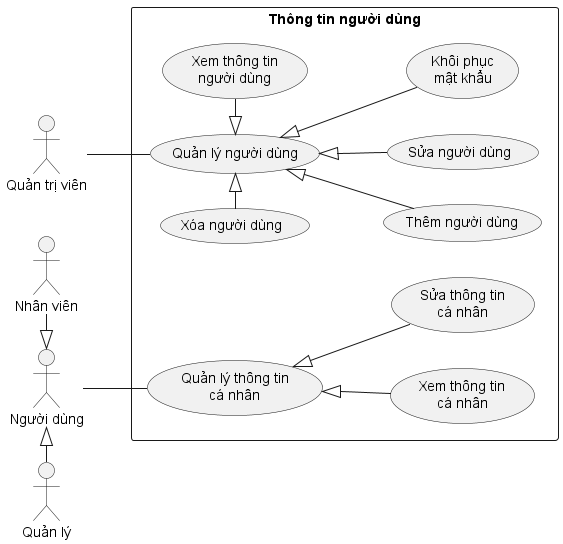
\includegraphics[width=\textwidth]{Hinhve/usecases/User}
    \caption{Biểu đồ use case phân rã Thông tin người dùng}
    \label{fig:uc-user}
\end{figure}
\break
% END OF SECTION

% START OF SECTION
\section{Đặc tả chức năng}
\label{section:uc-specification}
% Sinh viên lựa chọn từ 4 đến 7 use case quan trọng nhất của đồ án để đặc tả chi tiết. Mỗi đặc tả bao gồm ít nhất các thông tin sau: (i) Tên use case, (ii) Luồng sự kiện (chính và phát sinh), (iii) Tiền điều kiện, và (iv) Hậu điều kiện. Sinh viên chỉ vẽ bổ sung biểu đồ hoạt động khi đặc tả use case phức tạp.


\subsection{Đặc tả use case Xác thực người dùng}
\label{section:uc-authentication}
Bảng \ref{table:uc-authentication} mô tả chi tiết use case Xác thực người dùng. Hình \ref{figure:sd-authentication} mô tả biểu đồ tuần tự của use case này.
\begin{table}[H]
    \begin{tabularx}{\textwidth}{|l|c|X|X|}
        \hline
        \textbf{Mã Use case}                     & \multicolumn{3}{l|}{UC00}                                                                                                                             \\ \hline
        \textbf{Tên Use case}                    & \multicolumn{3}{l|}{Xác thực người dùng}                                                                                                              \\ \hline
        \textbf{Tác nhân}                        & \multicolumn{3}{l|}{Quản trị viên, Nhân viên, Quản lý}                                                                                                \\ \hline
        \textbf{Mô tả}                           & \multicolumn{3}{l|}{Người dùng muốn đăng nhập, đăng xuất}                                                                                             \\ \hline
        \textbf{Tiền điều kiện}                  & \multicolumn{3}{l|}{Có tài khoản trong hệ thống}                                                                                                      \\ \hline
        \multirow{3}{*}{\textbf{Luồng sự kiện}}  & \multicolumn{1}{c|}{\textbf{STT}}                         & \multicolumn{1}{c|}{\textbf{Hành động}} & \multicolumn{1}{c|}{\textbf{Hệ thống phản hồi}} \\ \cline{2-4}
                                                 & \multirow{1}{*}{\textbf{1}}                               & Nhập tên, mật khẩu                      & Hiện trang chính                                \\ \cline{2-4}
                                                 & \multirow{1}{*}{\textbf{2}}                               & Chọn nút đăng xuất                      & Hiện trang đăng nhập                            \\ \hline
        \multirow{2}{*}{\textbf{Luồng ngoại lệ}} & \multicolumn{1}{c|}{\textbf{STT}}                         & \multicolumn{1}{c|}{\textbf{Hành động}} & \multicolumn{1}{c|}{\textbf{Hệ thống phản hồi}} \\ \cline{2-4}
                                                 & \multirow{1}{*}{\textbf{1}}                               & Nhập tên, mật khẩu                      & Thông báo sai thông tin                         \\ \hline
        \textbf{Hậu điều kiện}                   & \multicolumn{3}{l|}{Đăng nhập hoặc đăng xuất thành công}                                                                                              \\ \hline
    \end{tabularx}
    \caption{Đặc tả use case Xác thực người dùng}
    \label{table:uc-authentication}
\end{table}

\begin{figure}[H]
    \centering
    \includegraphics[width=0.65\textwidth]{Hinhve/sequences/Authentication.png}
    \caption{Biểu đồ tuần tự use case Xác thực người dùng}
    \label{figure:sd-authentication}
\end{figure}
\break


\subsection{Đặc tả use case Lọc và xem sản phẩm}
\label{section:uc-product-filter}
Bảng \ref{table:uc-product-filter} mô tả chi tiết use case Lọc và xem sản phẩm. Hình \ref{figure:sd-product-filter} mô tả biểu đồ tuần tự của use case này.
\begin{table}[H]
    \begin{tabular}{|l|c|l|l|}
        \hline
        \textbf{Mã Use case}                    & \multicolumn{3}{l|}{UC10}                                                                                                                                       \\ \hline
        \textbf{Tên Use case}                   & \multicolumn{3}{l|}{Lọc và xem sản phẩm}                                                                                                                        \\ \hline
        \textbf{Tác nhân}                       & \multicolumn{3}{l|}{Nhân viên, Quản lý}                                                                                                                         \\ \hline
        \multirow{2}{*}{\textbf{Mô tả} }        & \multicolumn{3}{l|}{Người dùng muốn lọc bằng tên, mã vạch, sắp xếp}                                                                                             \\
                                                & \multicolumn{3}{l|}{và xem thông tin}                                                                                                                           \\ \hline
        \textbf{Tiền điều kiện}                 & \multicolumn{3}{l|}{Người dùng là Nhân viên hoặc Quản lý}                                                                                                       \\ \hline
        \multirow{7}{*}{\textbf{Luồng sự kiện}} & \multicolumn{1}{c|}{\textbf{STT}}                                   & \multicolumn{1}{c|}{\textbf{Hành động}} & \multicolumn{1}{c|}{\textbf{Hệ thống phản hồi}} \\ \cline{2-4}
                                                & \multirow{6}{*}{\textbf{1}}                                         & Chọn nút hình kính lúp                  & Hiện form lọc                                   \\ \cline{3-4}
                                                &                                                                     & Điền dữ liệu                            &                                                 \\
                                                &                                                                     & Có thể chọn nút hình                    & Điền mã vạch vào                                \\
                                                &                                                                     & mã vạch để quét mã vạch                 & trường dữ liệu                                  \\ \cline{3-4}
                                                &                                                                     & Chọn nút 'Tìm kiếm'                     & Hiện màn danh sách                              \\ \cline{3-4}
                                                &                                                                     & Chọn ô thông tin sản phẩm               & Hiện màn thông tin                              \\ \hline
        \textbf{Hậu điều kiện}                  & \multicolumn{3}{l|}{Lọc và Hiện chi tiết thông tin}                                                                                                             \\ \hline
    \end{tabular}
    \caption{Đặc tả use case Lọc và xem sản phẩm}
    \label{table:uc-product-filter}
\end{table}
\begin{figure}[H]
    \centering
    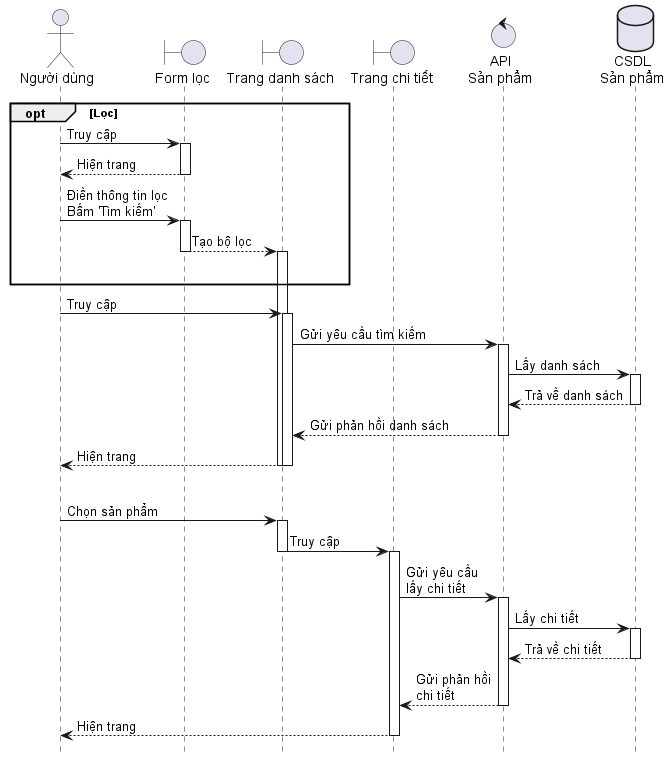
\includegraphics[width=0.7\textwidth]{Hinhve/sequences/ProductFilter.png}
    \caption{Biểu đồ tuần tự use case Lọc và xem sản phẩm}
    \label{figure:sd-product-filter}
\end{figure}
\break


\subsection{Đặc tả use case Quản lý sản phẩm}
\label{section:uc-product-manage}
Bảng \ref{table:uc-product-manage} mô tả chi tiết use case Quản lý sản phẩm. Hình \ref{figure:sd-product-manage} mô tả biểu đồ tuần tự của use case này.
\begin{figure}[H]
    \centering
    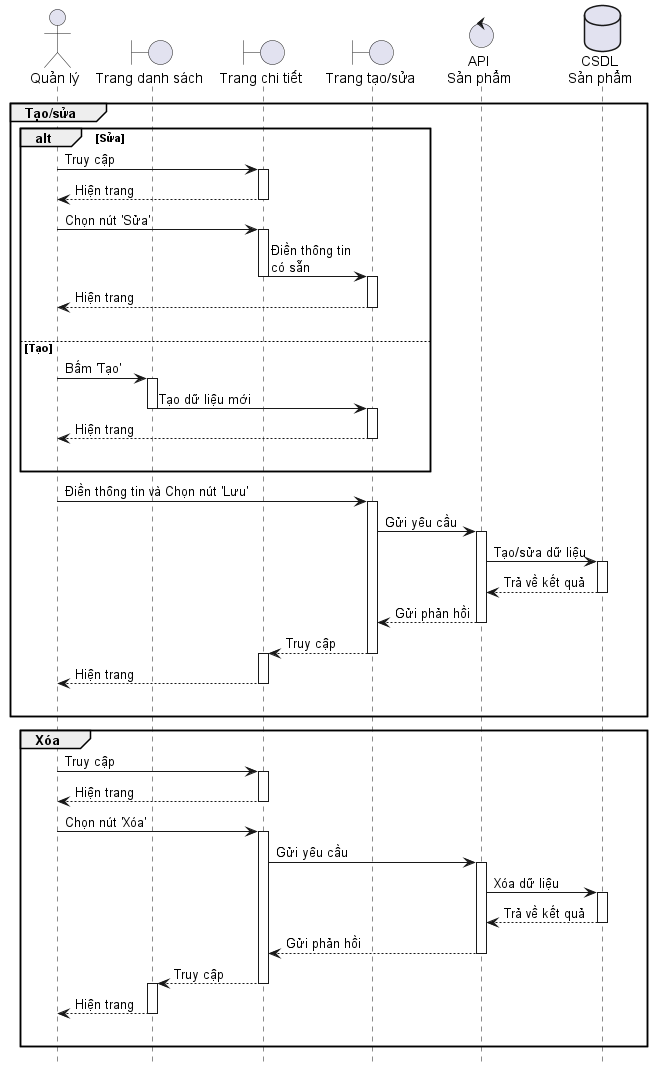
\includegraphics[width=0.9\textwidth]{Hinhve/sequences/ProductManage.png}
    \caption{Biểu đồ tuần tự use case Quản lý sản phẩm}
    \label{figure:sd-product-manage}
\end{figure}
\begin{table}[H]
    \begin{tabular}{|l|c|l|l|}
        \hline
        \textbf{Mã Use case}                    & \multicolumn{3}{l|}{UC11}                                                                                                                                  \\ \hline
        \textbf{Tên Use case}                   & \multicolumn{3}{l|}{Quản lý sản phẩm}                                                                                                                      \\ \hline
        \textbf{Tác nhân}                       & \multicolumn{3}{l|}{Quản lý}                                                                                                                               \\ \hline
        \textbf{Mô tả}                          & \multicolumn{3}{l|}{Người dùng muốn thêm, sửa, xóa sản phẩm}                                                                                               \\ \hline
        \textbf{Tiền điều kiện}                 & \multicolumn{3}{l|}{Người dùng là Quản lý}                                                                                                                 \\ \hline
        \multirow{9}{*}{\textbf{Luồng sự kiện}} & \multicolumn{1}{c|}{\textbf{STT}}                            & \multicolumn{1}{c|}{\textbf{Hành động}}   & \multicolumn{1}{c|}{\textbf{Hệ thống phản hồi}} \\ \cline{2-4}
                                                & \multirow{3}{*}{\textbf{1}}                                  & Chọn nút tạo mới ' + '                    & Hiện form tạo                                   \\ \cline{3-4}
                                                &                                                              & Điền thông tin                            &                                                 \\
                                                &                                                              & Chọn nút 'Lưu'                            & Hiện màn danh sách                              \\ \cline{2-4}
                                                & \multirow{4}{*}{\textbf{2}}                                  & Chọn ô thông tin sản phẩm                 & Hiện màn thông tin                              \\ \cline{3-4}
                                                &                                                              & Chọn nút ' \vdots{} ' $\rightarrow$ 'Sửa' & Hiện form sửa                                   \\ \cline{3-4}
                                                &                                                              & Điền thông tin                            &                                                 \\
                                                &                                                              & Chọn nút 'Lưu'                            & Hiện màn thông tin                              \\ \cline{2-4}
                                                & \multirow{1}{*}{\textbf{3}}                                  & Chọn nút ' \vdots{} ' $\rightarrow$ 'Xóa' & Hiện màn danh sách                              \\ \hline
        \textbf{Hậu điều kiện}                  & \multicolumn{3}{l|}{Thêm, sửa, xóa thông tin thành công}                                                                                                   \\ \hline
    \end{tabular}
    \caption{Đặc tả use case Quản lý sản phẩm}
    \label{table:uc-product-manage}
\end{table}


\subsection{Đặc tả use case Tìm kiếm sản phẩm}
\label{section:uc-product-search}
Bảng \ref{table:uc-product-search} mô tả chi tiết use case Tìm kiếm sản phẩm. Hình \ref{figure:sd-product-search} mô tả biểu đồ tuần tự của use case này.
\begin{table}[H]
    \begin{tabular}{|l|c|l|l|}
        \hline
        \textbf{Mã Use case}                    & \multicolumn{3}{l|}{UC12}                                                                                                                                      \\ \hline
        \textbf{Tên Use case}                   & \multicolumn{3}{l|}{Tìm kiếm sản phẩm}                                                                                                                         \\ \hline
        \textbf{Tác nhân}                       & \multicolumn{3}{l|}{Nhân viên, Quản lý}                                                                                                                        \\ \hline
        \multirow{2}{*}{\textbf{Mô tả} }        & \multicolumn{3}{l|}{Người dùng muốn tìm kiếm sản phẩm để thêm vào}                                                                                             \\
                                                & \multicolumn{3}{l|}{đơn từ}                                                                                                                                    \\ \hline
        \textbf{Tiền điều kiện}                 & \multicolumn{3}{l|}{Người dùng là Nhân viên hoặc Quản lý}                                                                                                      \\ \hline
        \multirow{6}{*}{\textbf{Luồng sự kiện}} & \multicolumn{1}{c|}{\textbf{STT}}                                  & \multicolumn{1}{c|}{\textbf{Hành động}} & \multicolumn{1}{c|}{\textbf{Hệ thống phản hồi}} \\ \cline{2-4}
                                                & \multirow{5}{*}{\textbf{1}}                                        & Chọn nút '+ Thêm'                       & Hiện màn tìm kiếm                               \\ \cline{3-4}
                                                &                                                                    & Điền tên hoặc mã vạch                   &                                                 \\
                                                &                                                                    & Có thể chọn nút hình                    & Điền mã vạch vào                                \\
                                                &                                                                    & mã vạch để quét mã vạch                 & trường dữ liệu                                  \\ \cline{3-4}
                                                &                                                                    & Chọn nút 'Tìm kiếm'                     & Hiện chuỗi danh sách                            \\ \cline{3-4}
                                                &                                                                    & Chọn ô thông tin sản phẩm               & Quay về màn đơn từ                              \\ \hline
        \textbf{Hậu điều kiện}                  & \multicolumn{3}{l|}{Tìm kiếm và thêm sản phẩm vào đơn từ}                                                                                                      \\ \hline
    \end{tabular}
    \caption{Đặc tả use case Tìm kiếm sản phẩm}
    \label{table:uc-product-search}
\end{table}
\break

\begin{figure}[H]
    \centering
    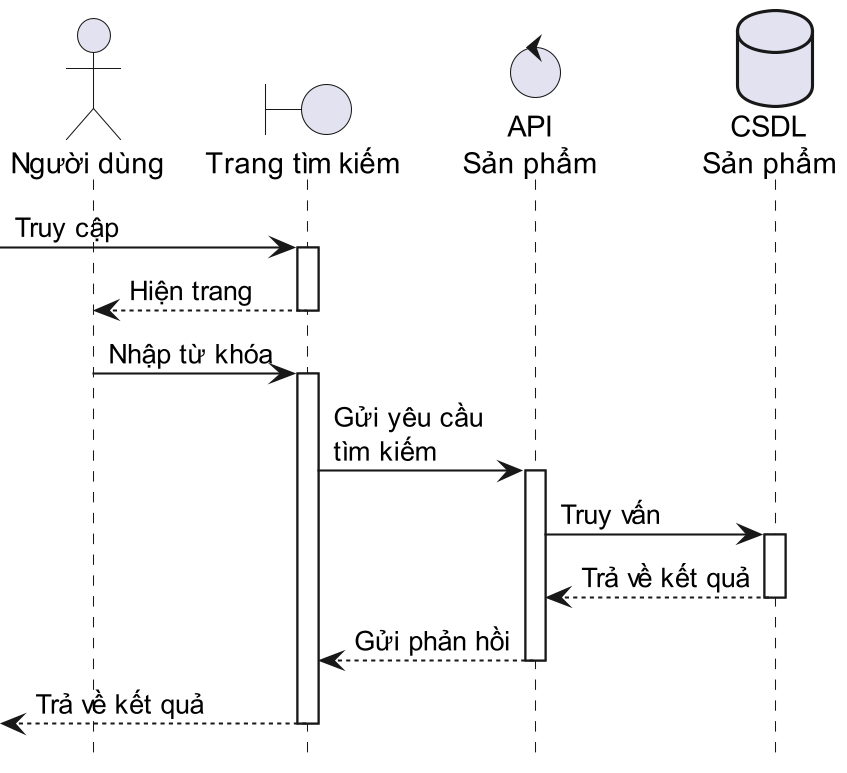
\includegraphics[width=0.9\textwidth]{Hinhve/sequences/ProductSearch.png}
    \caption{Biểu đồ tuần tự use case Tìm kiếm sản phẩm}
    \label{figure:sd-product-search}
\end{figure}


\subsection{Đặc tả use case Lọc và xem phiếu nhập kho}
\label{section:uc-importreport-filter}
Bảng \ref{table:uc-importreport-filter} mô tả chi tiết use case Lọc và xem phiếu nhập kho. Hình \ref{figure:sd-importreport-filter} mô tả biểu đồ tuần tự của use case này.
\begin{table}[H]
    \begin{tabular}{|l|c|l|l|}
        \hline
        \textbf{Mã Use case}                    & \multicolumn{3}{l|}{UC20}                                                                                                                                                   \\ \hline
        \textbf{Tên Use case}                   & \multicolumn{3}{l|}{Lọc và xem phiếu nhập kho}                                                                                                                              \\ \hline
        \textbf{Tác nhân}                       & \multicolumn{3}{l|}{Quản lý}                                                                                                                                                \\ \hline
        \multirow{2}{*}{\textbf{Mô tả} }        & \multicolumn{3}{l|}{Người dùng muốn lọc bằng tên, mã vạch, ngày tháng, sắp xếp}                                                                                             \\
                                                & \multicolumn{3}{l|}{và xem thông tin}                                                                                                                                       \\ \hline
        \textbf{Tiền điều kiện}                 & \multicolumn{3}{l|}{Người dùng là Quản lý}                                                                                                                                  \\ \hline
        \multirow{7}{*}{\textbf{Luồng sự kiện}} & \multicolumn{1}{c|}{\textbf{STT}}                                               & \multicolumn{1}{c|}{\textbf{Hành động}} & \multicolumn{1}{c|}{\textbf{Hệ thống phản hồi}} \\ \cline{2-4}
                                                & \multirow{6}{*}{\textbf{1}}                                                     & Chọn nút hình kính lúp                  & Hiện form lọc                                   \\ \cline{3-4}
                                                &                                                                                 & Điền dữ liệu                            &                                                 \\
                                                &                                                                                 & Có thể chọn nút hình                    & Điền mã vạch vào                                \\
                                                &                                                                                 & mã vạch để quét mã vạch                 & trường dữ liệu                                  \\ \cline{3-4}
                                                &                                                                                 & Chọn nút 'Tìm kiếm'                     & Hiện màn danh sách                              \\ \cline{3-4}
                                                &                                                                                 & Chọn ô thông tin phiếu đơn              & Hiện màn thông tin                              \\ \hline
        \textbf{Hậu điều kiện}                  & \multicolumn{3}{l|}{Lọc và Hiện chi tiết thông tin}                                                                                                                         \\ \hline
    \end{tabular}
    \caption{Đặc tả use case Lọc và xem phiếu nhập kho}
    \label{table:uc-importreport-filter}
\end{table}
\break

\begin{figure}[H]
    \centering
    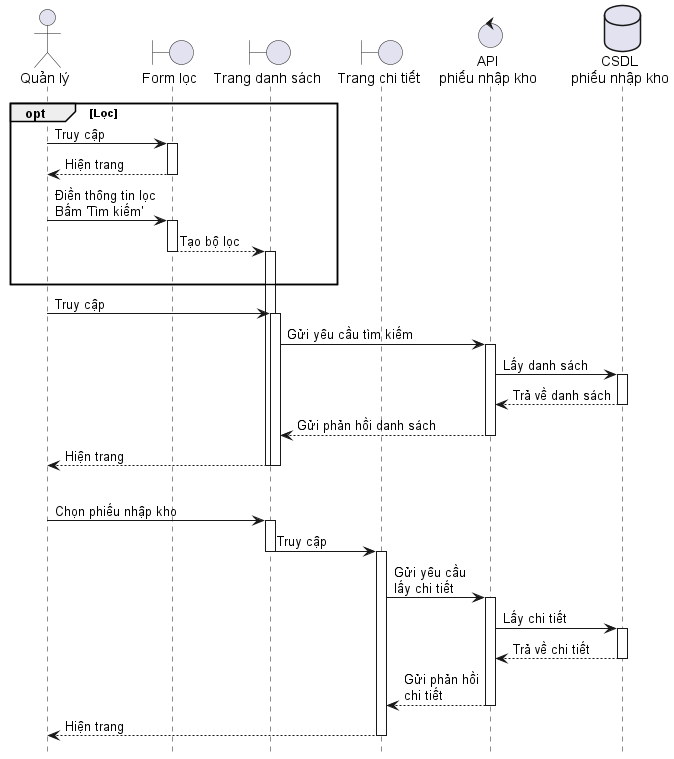
\includegraphics[width=1\textwidth]{Hinhve/sequences/ImportReportFilter.png}
    \caption{Biểu đồ tuần tự use case Lọc và xem phiếu nhập kho}
    \label{figure:sd-importreport-filter}
\end{figure}
\break


\subsection{Đặc tả use case Quản lý phiếu nhập kho}
\label{section:uc-importreport-manage}
Bảng \ref{table:uc-importreport-manage} mô tả chi tiết use case Quản lý phiếu nhập kho. Hình \ref{figure:sd-importreport-manage} mô tả biểu đồ tuần tự của use case này.
\begin{figure}[H]
    \centering
    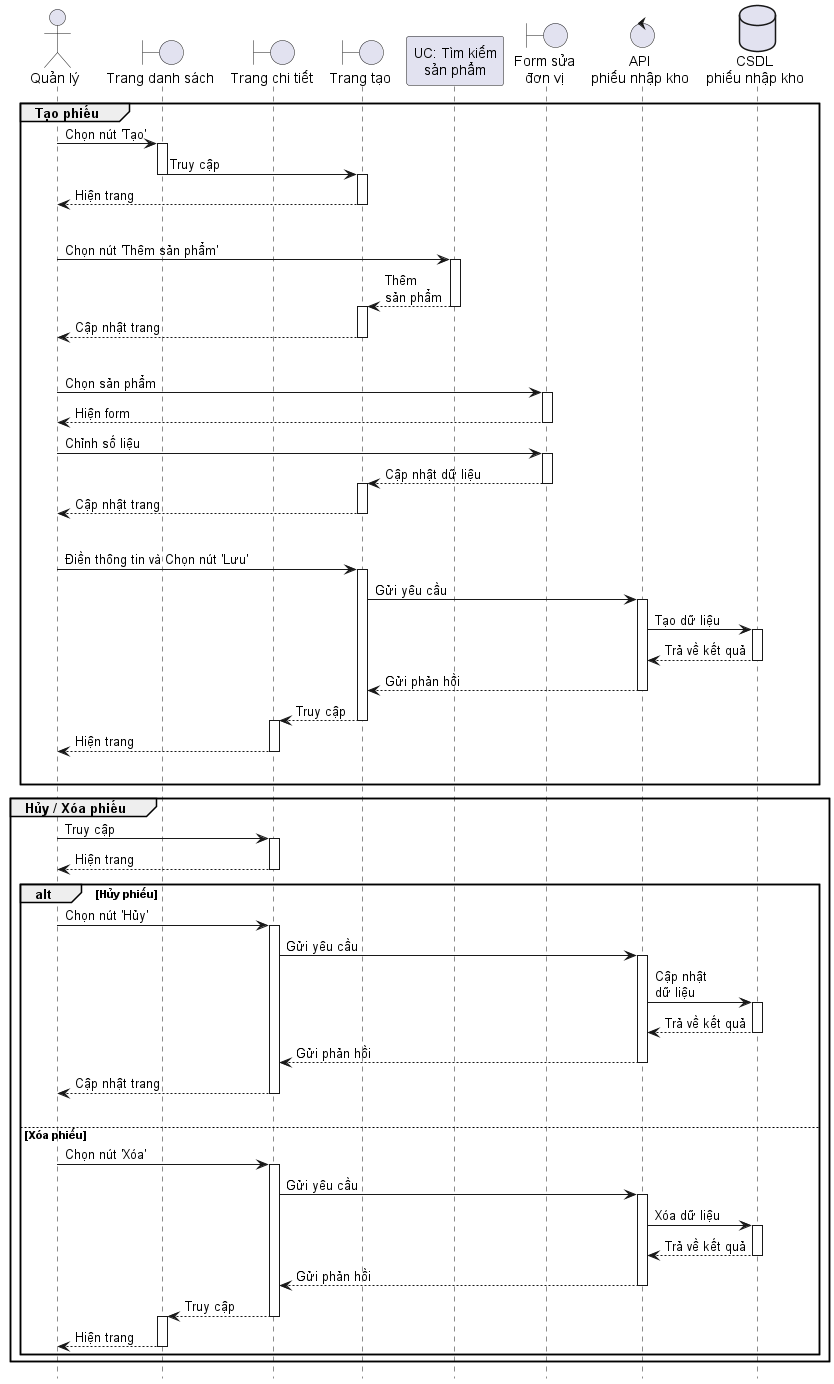
\includegraphics[width=0.85\textwidth]{Hinhve/sequences/ImportReportManage.png}
    \caption{Biểu đồ tuần tự use case Quản lý phiếu nhập kho}
    \label{figure:sd-importreport-manage}
\end{figure}
\break

\begin{table}[H]
    \begin{tabular}{|l|c|l|l|}
        \hline
        \textbf{Mã Use case}                     & \multicolumn{3}{l|}{UC21}                                                                                                                                        \\ \hline
        \textbf{Tên Use case}                    & \multicolumn{3}{l|}{Quản lý phiếu nhập kho}                                                                                                                      \\ \hline
        \textbf{Tác nhân}                        & \multicolumn{3}{l|}{Quản lý}                                                                                                                                     \\ \hline
        \textbf{Mô tả}                           & \multicolumn{3}{l|}{Người dùng muốn thêm, hủy, xóa phiếu nhập kho}                                                                                               \\ \hline
        \textbf{Tiền điều kiện}                  & \multicolumn{3}{l|}{Người dùng là Quản lý}                                                                                                                       \\ \hline
        \multirow{14}{*}{\textbf{Luồng sự kiện}} & \multicolumn{1}{c|}{\textbf{STT}}                                  & \multicolumn{1}{c|}{\textbf{Hành động}}   & \multicolumn{1}{c|}{\textbf{Hệ thống phản hồi}} \\ \cline{2-4}
                                                 & \multirow{10}{*}{\textbf{1}}                                       & Chọn nút tạo mới ' + '                    & Hiện form tạo                                   \\ \cline{3-4}
                                                 &                                                                    & Chọn nút '+ Thêm' để                      & Hiện màn tìm kiếm                               \\
                                                 &                                                                    & thêm sản phẩm vào phiếu                   & sản phẩm                                        \\ \cline{3-4}
                                                 &                                                                    & Sau khi chọn sản phẩm,                    & Hiện form chỉnh                                 \\
                                                 &                                                                    & chọn ô thông tin sản phẩm                 & số lượng, giá nhập                              \\ \cline{3-4}
                                                 &                                                                    & Có thể quẹt trái để xóa                   & Xóa mục sản phẩm                                \\ \cline{3-4}
                                                 &                                                                    & Có thể quẹt phải để xem                   & Hiện màn thông tin                              \\
                                                 &                                                                    & chi tiết sản phẩm                         & sản phẩm                                        \\ \cline{3-4}
                                                 &                                                                    & Có thể chọn nút 'Xóa'                     & Xóa hết mục sản phẩm                            \\ \cline{3-4}
                                                 &                                                                    & Chọn nút 'Lưu'                            & Hiện màn danh sách                              \\ \cline{2-4}
                                                 & \multirow{2}{*}{\textbf{2}}                                        & Chọn ô thông tin phiếu đơn                & Hiện màn thông tin                              \\ \cline{3-4}
                                                 &                                                                    & Chọn nút ' \vdots{} ' $\rightarrow$ 'Hủy' & Cập nhật thông tin                              \\ \cline{2-4}
                                                 & \multirow{1}{*}{\textbf{3}}                                        & Chọn nút ' \vdots{} ' $\rightarrow$ 'Xóa' & Hiện màn danh sách                              \\ \hline
        \multirow{3}{*}{\textbf{Luồng ngoại lệ}} & \multicolumn{1}{c|}{\textbf{STT}}                                  & \multicolumn{1}{c|}{\textbf{Hành động}}   & \multicolumn{1}{c|}{\textbf{Hệ thống phản hồi}} \\ \cline{2-4}
                                                 & \multirow{2}{*}{\textbf{1}}                                        & Sau khi chọn sản phẩm                     & Thông báo đã tồn tại                            \\
                                                 &                                                                    &                                           & sản phẩm trong đơn                              \\ \hline
        \textbf{Hậu điều kiện}                   & \multicolumn{3}{l|}{Thêm, hủy, xóa phiếu đơn thành công}                                                                                                         \\ \hline
    \end{tabular}
    \caption{Đặc tả use case Quản lý phiếu nhập kho}
    \label{table:uc-importreport-manage}
\end{table}


\subsection{Đặc tả use case Lọc và xem phiếu xuất kho}
\label{section:uc-exportreport-filter}
Bảng \ref{table:uc-exportreport-filter}, Hình \ref{figure:sd-exportreport-filter} mô tả chi tiết use case Lọc và xem phiếu xuất kho.
\begin{table}[H]
    \begin{tabular}{|l|c|l|l|}
        \hline
        \textbf{Mã Use case}                    & \multicolumn{3}{l|}{UC30}                                                                                                                                                   \\ \hline
        \textbf{Tên Use case}                   & \multicolumn{3}{l|}{Lọc và xem phiếu xuất kho}                                                                                                                              \\ \hline
        \textbf{Tác nhân}                       & \multicolumn{3}{l|}{Quản lý}                                                                                                                                                \\ \hline
        \multirow{2}{*}{\textbf{Mô tả} }        & \multicolumn{3}{l|}{Người dùng muốn lọc bằng tên, mã vạch, ngày tháng, sắp xếp}                                                                                             \\
                                                & \multicolumn{3}{l|}{và xem thông tin}                                                                                                                                       \\ \hline
        \textbf{Tiền điều kiện}                 & \multicolumn{3}{l|}{Người dùng là Quản lý}                                                                                                                                  \\ \hline
        \multirow{7}{*}{\textbf{Luồng sự kiện}} & \multicolumn{1}{c|}{\textbf{STT}}                                               & \multicolumn{1}{c|}{\textbf{Hành động}} & \multicolumn{1}{c|}{\textbf{Hệ thống phản hồi}} \\ \cline{2-4}
                                                & \multirow{6}{*}{\textbf{1}}                                                     & Chọn nút hình kính lúp                  & Hiện form lọc                                   \\ \cline{3-4}
                                                &                                                                                 & Điền dữ liệu                            &                                                 \\
                                                &                                                                                 & Có thể chọn nút hình                    & Điền mã vạch vào                                \\
                                                &                                                                                 & mã vạch để quét mã vạch                 & trường dữ liệu                                  \\ \cline{3-4}
                                                &                                                                                 & Chọn nút 'Tìm kiếm'                     & Hiện màn danh sách                              \\ \cline{3-4}
                                                &                                                                                 & Chọn ô thông tin phiếu đơn              & Hiện màn thông tin                              \\ \hline
        \textbf{Hậu điều kiện}                  & \multicolumn{3}{l|}{Lọc và Hiện chi tiết thông tin}                                                                                                                         \\ \hline
    \end{tabular}
    \caption{Đặc tả use case Lọc và xem phiếu xuất kho}
    \label{table:uc-exportreport-filter}
\end{table}
\break

\begin{figure}[H]
    \centering
    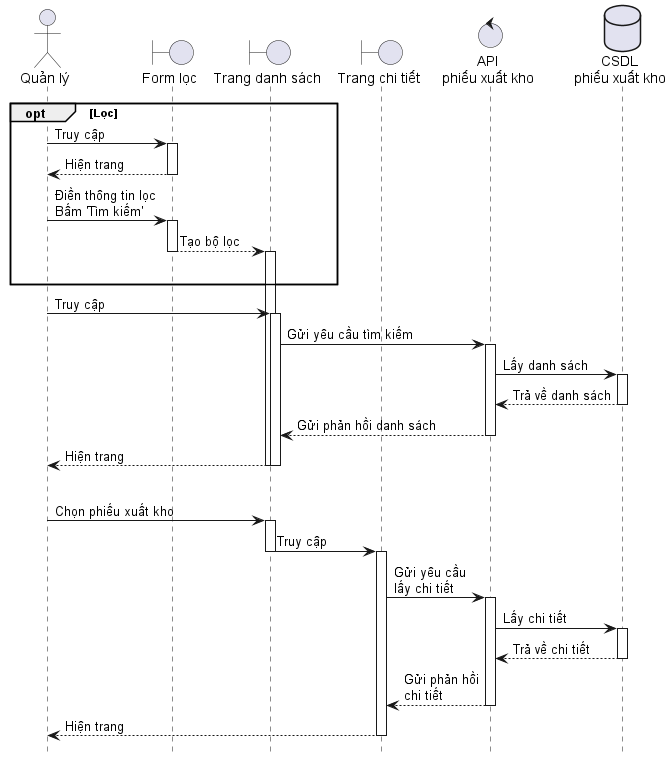
\includegraphics[width=1\textwidth]{Hinhve/sequences/ExportReportFilter.png}
    \caption{Biểu đồ tuần tự use case Lọc và xem phiếu xuất kho}
    \label{figure:sd-exportreport-filter}
\end{figure}
\break


\subsection{Đặc tả use case Quản lý phiếu xuất kho}
\label{section:uc-exportreport-manage}
Bảng \ref{table:uc-exportreport-manage} mô tả chi tiết use case Quản lý phiếu xuất kho. Hình \ref{figure:sd-exportreport-manage} mô tả biểu đồ tuần tự của use case này.
\begin{table}[H]
    \begin{tabular}{|l|c|l|l|}
        \hline
        \textbf{Mã Use case}                     & \multicolumn{3}{l|}{UC31}                                                                                                                                        \\ \hline
        \textbf{Tên Use case}                    & \multicolumn{3}{l|}{Quản lý phiếu xuất kho}                                                                                                                      \\ \hline
        \textbf{Tác nhân}                        & \multicolumn{3}{l|}{Quản lý}                                                                                                                                     \\ \hline
        \textbf{Mô tả}                           & \multicolumn{3}{l|}{Người dùng muốn thêm, hủy, xóa phiếu xuất kho}                                                                                               \\ \hline
        \textbf{Tiền điều kiện}                  & \multicolumn{3}{l|}{Người dùng là Quản lý}                                                                                                                       \\ \hline
        \multirow{14}{*}{\textbf{Luồng sự kiện}} & \multicolumn{1}{c|}{\textbf{STT}}                                  & \multicolumn{1}{c|}{\textbf{Hành động}}   & \multicolumn{1}{c|}{\textbf{Hệ thống phản hồi}} \\ \cline{2-4}
                                                 & \multirow{10}{*}{\textbf{1}}                                       & Chọn nút tạo mới ' + '                    & Hiện form tạo                                   \\ \cline{3-4}
                                                 &                                                                    & Chọn nút '+ Thêm' để                      & Hiện màn tìm kiếm                               \\
                                                 &                                                                    & thêm sản phẩm vào phiếu                   & sản phẩm                                        \\ \cline{3-4}
                                                 &                                                                    & Sau khi chọn sản phẩm,                    & Hiện form chỉnh                                 \\
                                                 &                                                                    & chọn ô thông tin sản phẩm                 & số lượng                                        \\ \cline{3-4}
                                                 &                                                                    & Có thể quẹt trái để xóa                   & Xóa mục sản phẩm                                \\ \cline{3-4}
                                                 &                                                                    & Có thể quẹt phải để xem                   & Hiện màn thông tin                              \\
                                                 &                                                                    & chi tiết sản phẩm                         & sản phẩm                                        \\ \cline{3-4}
                                                 &                                                                    & Có thể chọn nút 'Xóa'                     & Xóa hết mục sản phẩm                            \\ \cline{3-4}
                                                 &                                                                    & Chọn nút 'Lưu'                            & Hiện màn danh sách                              \\ \cline{2-4}
                                                 & \multirow{2}{*}{\textbf{2}}                                        & Chọn ô thông tin phiếu đơn                & Hiện màn thông tin                              \\ \cline{3-4}
                                                 &                                                                    & Chọn nút ' \vdots{} ' $\rightarrow$ 'Hủy' & Cập nhật thông tin                              \\ \cline{2-4}
                                                 & \multirow{1}{*}{\textbf{3}}                                        & Chọn nút ' \vdots{} ' $\rightarrow$ 'Xóa' & Hiện màn danh sách                              \\ \hline
        \multirow{7}{*}{\textbf{Luồng ngoại lệ}} & \multicolumn{1}{c|}{\textbf{STT}}                                  & \multicolumn{1}{c|}{\textbf{Hành động}}   & \multicolumn{1}{c|}{\textbf{Hệ thống phản hồi}} \\ \cline{2-4}
                                                 & \multirow{6}{*}{\textbf{1}}                                        & Chọn nút '+ Thêm' để                      & Hiện màn tìm kiếm                               \\
                                                 &                                                                    & thêm sản phẩm vào đơn                     & sản phẩm                                        \\ \cline{3-4}
                                                 &                                                                    & Sau khi chọn sản phẩm                     & Thông báo đã tồn tại                            \\
                                                 &                                                                    &                                           & sản phẩm trong đơn                              \\ \cline{4-4}
                                                 &                                                                    &                                           & Thông báo hết hàng                              \\
                                                 &                                                                    &                                           & sản phẩm trong kho                              \\ \hline
        \textbf{Hậu điều kiện}                   & \multicolumn{3}{l|}{Thêm, hủy, xóa phiếu đơn thành công}                                                                                                         \\ \hline
    \end{tabular}
    \caption{Đặc tả use case Quản lý phiếu xuất kho}
    \label{table:uc-exportreport-manage}
\end{table}
\vfill
\break

\begin{figure}[H]
    \centering
    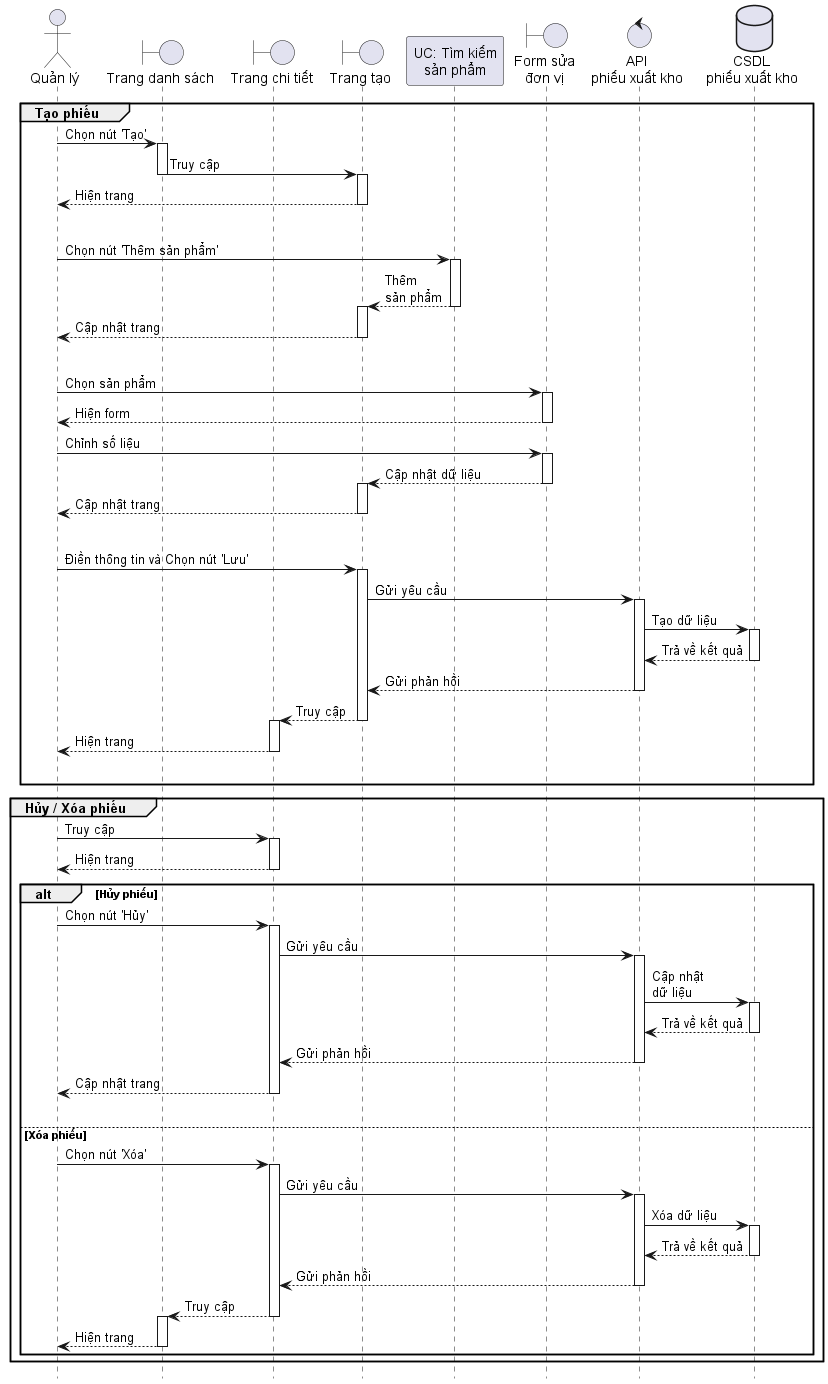
\includegraphics[width=0.9\textwidth]{Hinhve/sequences/ExportReportManage.png}
    \caption{Biểu đồ tuần tự use case Quản lý phiếu xuất kho}
    \label{figure:sd-exportreport-manage}
\end{figure}
\break


\subsection{Đặc tả use case Lọc và xem phiếu kiểm kho}
\label{section:uc-auditreport-filter}
Bảng \ref{table:uc-auditreport-filter} mô tả chi tiết use case Lọc và xem phiếu kiểm kho. Hình \ref{figure:sd-auditreport-filter} mô tả biểu đồ tuần tự của use case này.
\begin{table}[H]
    \begin{tabular}{|l|c|l|l|}
        \hline
        \textbf{Mã Use case}                    & \multicolumn{3}{l|}{UC40}                                                                                                                                                   \\ \hline
        \textbf{Tên Use case}                   & \multicolumn{3}{l|}{Lọc và xem phiếu kiểm kho}                                                                                                                              \\ \hline
        \textbf{Tác nhân}                       & \multicolumn{3}{l|}{Quản lý}                                                                                                                                                \\ \hline
        \multirow{2}{*}{\textbf{Mô tả} }        & \multicolumn{3}{l|}{Người dùng muốn lọc bằng tên, mã vạch, ngày tháng, sắp xếp}                                                                                             \\
                                                & \multicolumn{3}{l|}{và xem thông tin}                                                                                                                                       \\ \hline
        \textbf{Tiền điều kiện}                 & \multicolumn{3}{l|}{Người dùng là Quản lý}                                                                                                                                  \\ \hline
        \multirow{7}{*}{\textbf{Luồng sự kiện}} & \multicolumn{1}{c|}{\textbf{STT}}                                               & \multicolumn{1}{c|}{\textbf{Hành động}} & \multicolumn{1}{c|}{\textbf{Hệ thống phản hồi}} \\ \cline{2-4}
                                                & \multirow{6}{*}{\textbf{1}}                                                     & Chọn nút hình kính lúp                  & Hiện form lọc                                   \\ \cline{3-4}
                                                &                                                                                 & Điền dữ liệu                            &                                                 \\
                                                &                                                                                 & Có thể chọn nút hình                    & Điền mã vạch vào                                \\
                                                &                                                                                 & mã vạch để quét mã vạch                 & trường dữ liệu                                  \\ \cline{3-4}
                                                &                                                                                 & Chọn nút 'Tìm kiếm'                     & Hiện màn danh sách                              \\ \cline{3-4}
                                                &                                                                                 & Chọn ô thông tin phiếu đơn              & Hiện màn thông tin                              \\ \hline
        \textbf{Hậu điều kiện}                  & \multicolumn{3}{l|}{Lọc và Hiện chi tiết thông tin}                                                                                                                         \\ \hline
    \end{tabular}
    \caption{Đặc tả use case Lọc và xem phiếu kiểm kho}
    \label{table:uc-auditreport-filter}
\end{table}
\begin{figure}[H]
    \centering
    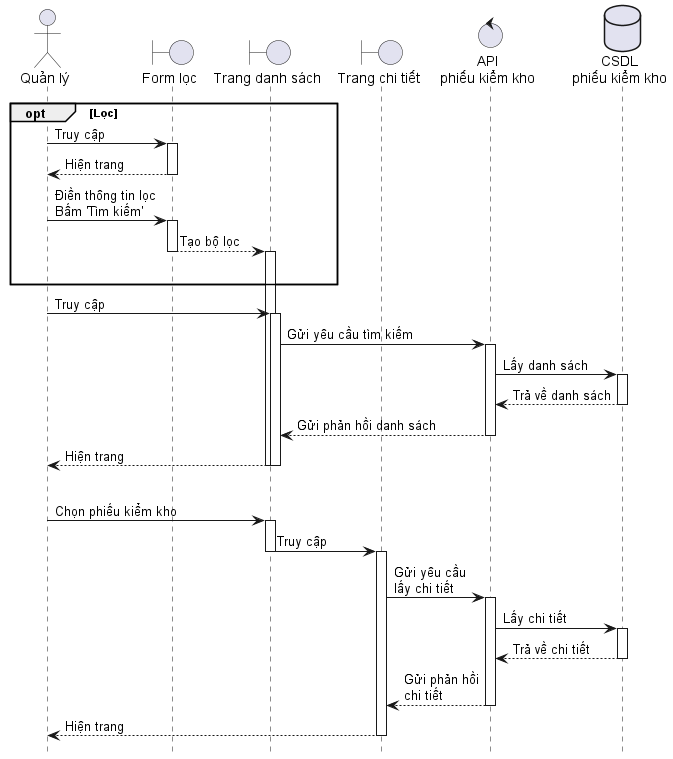
\includegraphics[width=0.7\textwidth]{Hinhve/sequences/AuditReportFilter.png}
    \caption{Biểu đồ tuần tự use case Lọc và xem phiếu kiểm kho}
    \label{figure:sd-auditreport-filter}
\end{figure}
\break


\subsection{Đặc tả use case Quản lý phiếu kiểm kho}
\label{section:uc-auditreport-manage}
Bảng \ref{table:uc-auditreport-manage} mô tả chi tiết use case Quản lý phiếu kiểm kho. Hình \ref{figure:sd-auditreport-manage} mô tả biểu đồ tuần tự của use case này.
\begin{table}[H]
    \begin{tabular}{|l|c|l|l|}
        \hline
        \textbf{Mã Use case}                     & \multicolumn{3}{l|}{UC41}                                                                                                                                   \\ \hline
        \textbf{Tên Use case}                    & \multicolumn{3}{l|}{Quản lý phiếu kiểm kho}                                                                                                                 \\ \hline
        \textbf{Tác nhân}                        & \multicolumn{3}{l|}{Quản lý}                                                                                                                                \\ \hline
        \textbf{Mô tả}                           & \multicolumn{3}{l|}{Người dùng muốn thêm, xóa phiếu kiểm kho}                                                                                               \\ \hline
        \textbf{Tiền điều kiện}                  & \multicolumn{3}{l|}{Người dùng là Quản lý}                                                                                                                  \\ \hline
        \multirow{14}{*}{\textbf{Luồng sự kiện}} & \multicolumn{1}{c|}{\textbf{STT}}                             & \multicolumn{1}{c|}{\textbf{Hành động}}   & \multicolumn{1}{c|}{\textbf{Hệ thống phản hồi}} \\ \cline{2-4}
                                                 & \multirow{10}{*}{\textbf{1}}                                  & Chọn nút tạo mới ' + '                    & Hiện form tạo                                   \\ \cline{3-4}
                                                 &                                                               & Chọn nút '+ Thêm' để                      & Hiện màn tìm kiếm                               \\
                                                 &                                                               & thêm sản phẩm vào phiếu                   & sản phẩm                                        \\ \cline{3-4}
                                                 &                                                               & Sau khi chọn sản phẩm,                    & Hiện form chỉnh                                 \\
                                                 &                                                               & chọn ô thông tin sản phẩm                 & số lượng chênh lệch                             \\ \cline{3-4}
                                                 &                                                               & Có thể quẹt trái để xóa                   & Xóa mục sản phẩm                                \\ \cline{3-4}
                                                 &                                                               & Có thể quẹt phải để xem                   & Hiện màn thông tin                              \\
                                                 &                                                               & chi tiết sản phẩm                         & sản phẩm                                        \\ \cline{3-4}
                                                 &                                                               & Có thể chọn nút 'Xóa'                     & Xóa hết mục sản phẩm                            \\ \cline{3-4}
                                                 &                                                               & Chọn nút 'Lưu'                            & Hiện màn danh sách                              \\ \cline{2-4}
                                                 & \multirow{2}{*}{\textbf{2}}                                   & Chọn ô thông tin phiếu đơn                & Hiện màn thông tin                              \\ \cline{3-4}
                                                 &                                                               & Chọn nút ' \vdots{} ' $\rightarrow$ 'Xóa' & Hiện màn danh sách                              \\ \hline
        \multirow{5}{*}{\textbf{Luồng ngoại lệ}} & \multicolumn{1}{c|}{\textbf{STT}}                             & \multicolumn{1}{c|}{\textbf{Hành động}}   & \multicolumn{1}{c|}{\textbf{Hệ thống phản hồi}} \\ \cline{2-4}
                                                 & \multirow{4}{*}{\textbf{1}}                                   & Chọn nút '+ Thêm' để                      & Hiện màn tìm kiếm                               \\
                                                 &                                                               & thêm sản phẩm vào đơn                     & sản phẩm                                        \\ \cline{3-4}
                                                 &                                                               & Sau khi chọn sản phẩm                     & Thông báo đã tồn tại                            \\
                                                 &                                                               &                                           & sản phẩm trong đơn                              \\ \hline
        \textbf{Hậu điều kiện}                   & \multicolumn{3}{l|}{Thêm, xóa phiếu đơn thành công}                                                                                                         \\ \hline
    \end{tabular}
    \caption{Đặc tả use case Quản lý phiếu kiểm kho}
    \label{table:uc-auditreport-manage}
\end{table}
\vfill
\break

\begin{figure}[H]
    \centering
    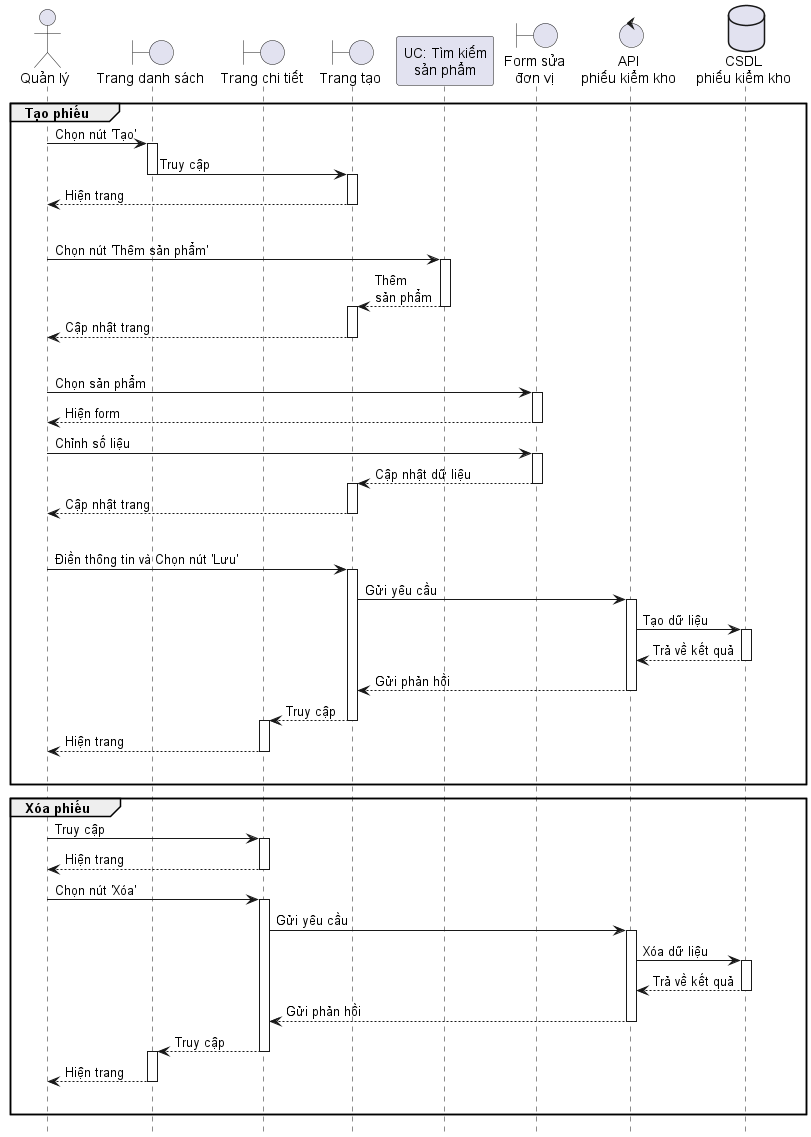
\includegraphics[width=1\textwidth]{Hinhve/sequences/AuditReportManage.png}
    \caption{Biểu đồ tuần tự use case Quản lý phiếu kiểm kho}
    \label{figure:sd-auditreport-manage}
\end{figure}
\break


\subsection{Đặc tả use case Lọc và xem hóa đơn}
\label{section:uc-invoice-filter}
Bảng \ref{table:uc-invoice-filter} mô tả chi tiết use case Lọc và xem hóa đơn. Hình \ref{figure:sd-invoice-filter} mô tả biểu đồ tuần tự của use case này.
\begin{table}[H]
    \begin{tabular}{|l|c|l|l|}
        \hline
        \textbf{Mã Use case}                    & \multicolumn{3}{l|}{UC50}                                                                                                                                          \\ \hline
        \textbf{Tên Use case}                   & \multicolumn{3}{l|}{Lọc và xem hóa đơn}                                                                                                                            \\ \hline
        \textbf{Tác nhân}                       & \multicolumn{3}{l|}{Nhân viên, Quản lý}                                                                                                                            \\ \hline
        \multirow{2}{*}{\textbf{Mô tả} }        & \multicolumn{3}{l|}{Người dùng muốn lọc bằng tên, mã vạch, trạng thái}                                                                                             \\
                                                & \multicolumn{3}{l|}{ngày tháng, sắp xếp và xem thông tin}                                                                                                          \\ \hline
        \textbf{Tiền điều kiện}                 & \multicolumn{3}{l|}{Người dùng là Nhân viên hoặc Quản lý}                                                                                                          \\ \hline
        \multirow{7}{*}{\textbf{Luồng sự kiện}} & \multicolumn{1}{c|}{\textbf{STT}}                                      & \multicolumn{1}{c|}{\textbf{Hành động}} & \multicolumn{1}{c|}{\textbf{Hệ thống phản hồi}} \\ \cline{2-4}
                                                & \multirow{6}{*}{\textbf{1}}                                            & Chọn nút hình kính lúp                  & Hiện form lọc                                   \\ \cline{3-4}
                                                &                                                                        & Điền dữ liệu                            &                                                 \\
                                                &                                                                        & Có thể chọn nút hình                    & Điền mã vạch vào                                \\
                                                &                                                                        & mã vạch để quét mã vạch                 & trường dữ liệu                                  \\ \cline{3-4}
                                                &                                                                        & Chọn nút 'Tìm kiếm'                     & Hiện màn danh sách                              \\ \cline{3-4}
                                                &                                                                        & Chọn ô thông tin hóa đơn                & Hiện màn thông tin                              \\ \hline
        \textbf{Hậu điều kiện}                  & \multicolumn{3}{l|}{Lọc và Hiện chi tiết thông tin}                                                                                                                \\ \hline
    \end{tabular}
    \caption{Đặc tả use case Lọc và xem hóa đơn}
    \label{table:uc-invoice-filter}
\end{table}
\begin{figure}[H]
    \centering
    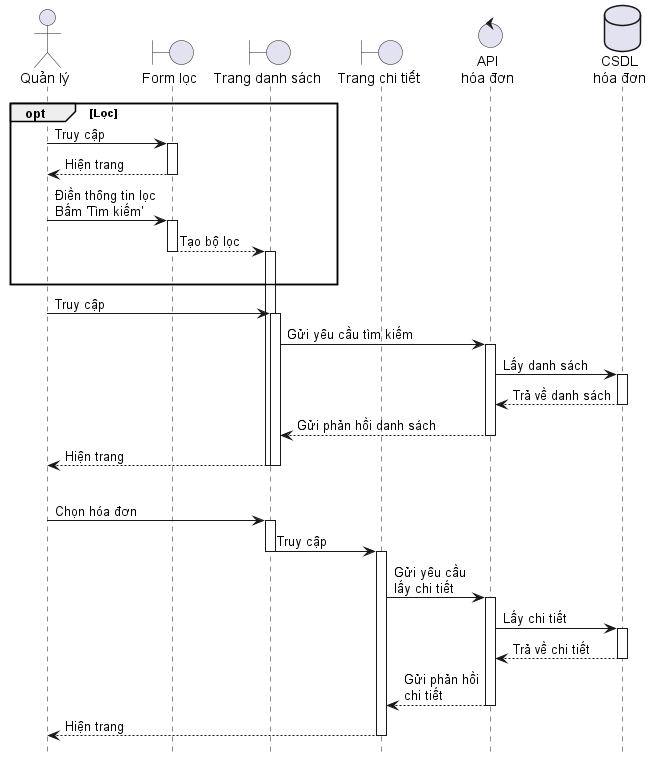
\includegraphics[width=0.7\textwidth]{Hinhve/sequences/InvoiceFilter.png}
    \caption{Biểu đồ tuần tự use case Lọc và xem hóa đơn}
    \label{figure:sd-invoice-filter}
\end{figure}
\break


\subsection{Đặc tả use case Quản lý hóa đơn}
\label{section:uc-invoice-manage}
Bảng \ref{table:uc-invoice-manage} mô tả chi tiết use case Quản lý hóa đơn. Hình \ref{figure:sd-invoice-manage1} và \ref{figure:sd-invoice-manage2} mô tả biểu đồ tuần tự của use case này.
\begin{table}[H]
    \begin{tabular}{|l|c|l|l|}
        \hline
        \textbf{Mã Use case}                     & \multicolumn{3}{l|}{UC51}                                                                                                                                             \\ \hline
        \textbf{Tên Use case}                    & \multicolumn{3}{l|}{Quản lý hóa đơn}                                                                                                                                  \\ \hline
        \textbf{Tác nhân}                        & \multicolumn{3}{l|}{Nhân viên, Quản lý}                                                                                                                               \\ \hline
        \textbf{Mô tả}                           & \multicolumn{3}{l|}{Người dùng muốn thêm, thanh toán, hủy, xóa hóa đơn}                                                                                               \\ \hline
        \textbf{Tiền điều kiện}                  & \multicolumn{3}{l|}{Người dùng là Nhân viên hoặc Quản lý}                                                                                                             \\ \hline
        \multirow{21}{*}{\textbf{Luồng sự kiện}} & \multicolumn{1}{c|}{\textbf{STT}}                                       & \multicolumn{1}{c|}{\textbf{Hành động}}   & \multicolumn{1}{c|}{\textbf{Hệ thống phản hồi}} \\ \cline{2-4}
                                                 & \multirow{15}{*}{\textbf{1}}                                            & Chọn nút tạo mới ' + '                    & Hiện form tạo                                   \\ \cline{3-4}
                                                 &                                                                         & Chọn nút '+ Thêm' để                      & Hiện màn tìm kiếm                               \\
                                                 &                                                                         & thêm sản phẩm vào đơn                     & sản phẩm                                        \\ \cline{3-4}
                                                 &                                                                         & Sau khi chọn sản phẩm,                    & Hiện form chỉnh                                 \\
                                                 &                                                                         & chọn ô thông tin sản phẩm                 & số lượng sản phẩm                               \\ \cline{3-4}
                                                 &                                                                         & Có thể quẹt trái để xóa                   & Xóa mục sản phẩm                                \\ \cline{3-4}
                                                 &                                                                         & Có thể quẹt phải để xem                   & Hiện màn thông tin                              \\
                                                 &                                                                         & chi tiết sản phẩm                         & sản phẩm                                        \\ \cline{3-4}
                                                 &                                                                         & Có thể chọn nút 'Xóa'                     & Xóa hết mục sản phẩm                            \\ \cline{3-4}
                                                 &                                                                         & Chọn thanh 'Khách hàng'                   & Hiện màn tìm kiếm                               \\
                                                 &                                                                         & để thêm vào hóa đơn                       & khách hàng                                      \\ \cline{3-4}
                                                 &                                                                         & Điền tổng tiền sẽ bán                     &                                                 \\
                                                 &                                                                         & Có thể tích ô để đánh dấu                 &                                                 \\
                                                 &                                                                         & thanh toán ngay                           &                                                 \\
                                                 &                                                                         & Chọn nút 'Lưu'                            & Hiện màn danh sách                              \\ \cline{2-4}
                                                 & \multirow{2}{*}{\textbf{2}}                                             & Chọn ô thông tin hóa đơn                  & Hiện màn thông tin                              \\ \cline{3-4}
                                                 &                                                                         & Chọn nút ' \vdots{} ' $\rightarrow$ 'Hủy' & Cập nhật thông tin                              \\ \cline{2-4}
                                                 & \multirow{2}{*}{\textbf{3}}                                             & Chọn nút                                  & Cập nhật thông tin                              \\
                                                 &                                                                         & ' \vdots{} ' $\rightarrow$ 'Thanh toán'   &                                                 \\ \cline{2-4}
                                                 & \multirow{1}{*}{\textbf{4}}                                             & Chọn nút ' \vdots{} ' $\rightarrow$ 'Xóa' & Hiện màn danh sách                              \\ \hline
        \multirow{7}{*}{\textbf{Luồng ngoại lệ}} & \multicolumn{1}{c|}{\textbf{STT}}                                       & \multicolumn{1}{c|}{\textbf{Hành động}}   & \multicolumn{1}{c|}{\textbf{Hệ thống phản hồi}} \\ \cline{2-4}
                                                 & \multirow{6}{*}{\textbf{1}}                                             & Chọn nút '+ Thêm' để                      & Hiện màn tìm kiếm                               \\
                                                 &                                                                         & thêm sản phẩm vào đơn                     & sản phẩm                                        \\ \cline{3-4}
                                                 &                                                                         & Sau khi chọn sản phẩm                     & Thông báo đã tồn tại                            \\
                                                 &                                                                         &                                           & sản phẩm trong đơn                              \\ \cline{4-4}
                                                 &                                                                         &                                           & Thông báo hết hàng                              \\
                                                 &                                                                         &                                           & sản phẩm trong kho                              \\ \hline
        \textbf{Hậu điều kiện}                   & \multicolumn{3}{l|}{Thêm, thanh toán, hủy, xóa hóa đơn thành công}                                                                                                    \\ \hline
    \end{tabular}
    \caption{Đặc tả use case Quản lý hóa đơn}
    \label{table:uc-invoice-manage}
\end{table}
\vfill
\break

\begin{figure}[H]
    \centering
    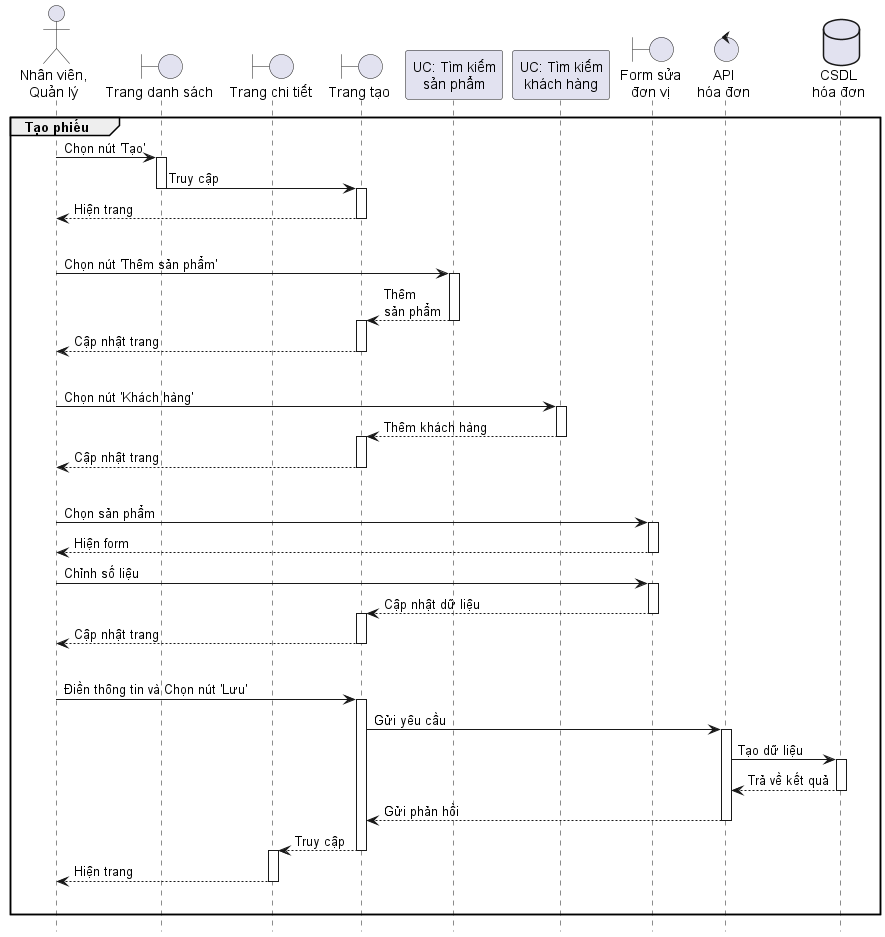
\includegraphics[width=1\textwidth]{Hinhve/sequences/InvoiceManage1.png}
    \caption{Biểu đồ tuần tự use case Quản lý hóa đơn (phần 1)}
    \label{figure:sd-invoice-manage1}
\end{figure}
\break

\begin{figure}[H]
    \centering
    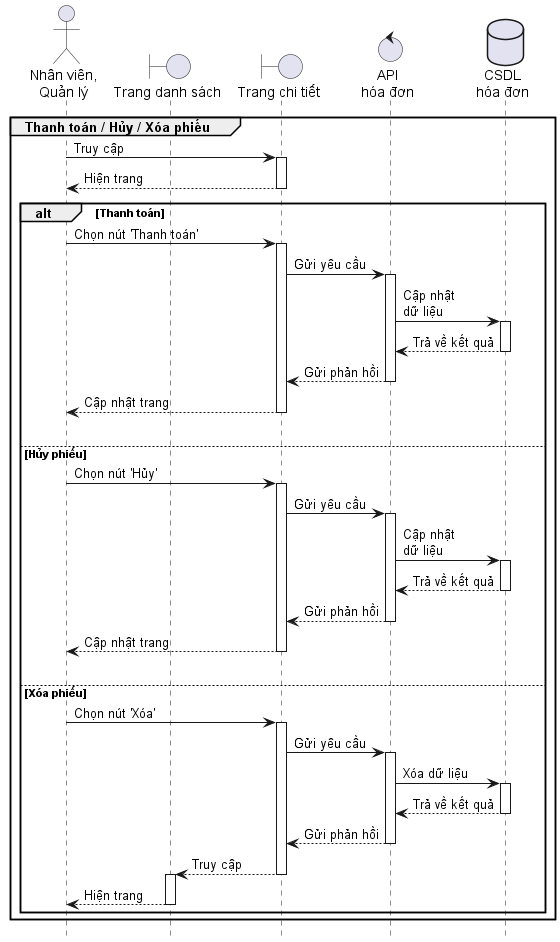
\includegraphics[width=1\textwidth]{Hinhve/sequences/InvoiceManage2.png}
    \caption{Biểu đồ tuần tự use case Quản lý hóa đơn (phần 2)}
    \label{figure:sd-invoice-manage2}
\end{figure}
\break


\subsection{Đặc tả use case Lọc và xem khách hàng}
\label{section:uc-client-filter}
Bảng \ref{table:uc-client-filter} mô tả chi tiết use case Lọc và xem khách hàng. Hình \ref{figure:sd-client-filter} mô tả biểu đồ tuần tự của use case này.
\begin{table}[H]
    \begin{tabular}{|l|c|l|l|}
        \hline
        \textbf{Mã Use case}                    & \multicolumn{3}{l|}{UC60}                                                                                                                                             \\ \hline
        \textbf{Tên Use case}                   & \multicolumn{3}{l|}{Lọc và xem khách hàng}                                                                                                                            \\ \hline
        \textbf{Tác nhân}                       & \multicolumn{3}{l|}{Nhân viên, Quản lý}                                                                                                                               \\ \hline
        \multirow{2}{*}{\textbf{Mô tả} }        & \multicolumn{3}{l|}{Người dùng muốn lọc bằng tên, số điện thoại, sắp xếp}                                                                                             \\
                                                & \multicolumn{3}{l|}{và xem chi tiết thông tin khách hàng}                                                                                                             \\ \hline
        \textbf{Tiền điều kiện}                 & \multicolumn{3}{l|}{Người dùng là Nhân viên hoặc Quản lý}                                                                                                             \\ \hline
        \multirow{7}{*}{\textbf{Luồng sự kiện}} & \multicolumn{1}{c|}{\textbf{STT}}                                         & \multicolumn{1}{c|}{\textbf{Hành động}} & \multicolumn{1}{c|}{\textbf{Hệ thống phản hồi}} \\ \cline{2-4}
                                                & \multirow{4}{*}{\textbf{1}}                                               & Chọn nút hình kính lúp                  & Hiện form lọc                                   \\ \cline{3-4}
                                                &                                                                           & Điền dữ liệu                            &                                                 \\
                                                &                                                                           & Chọn nút 'Tìm kiếm'                     & Hiện màn danh sách                              \\ \cline{3-4}
                                                &                                                                           & Chọn ô thông tin khách hàng             & Hiện màn thông tin                              \\ \hline
        \textbf{Hậu điều kiện}                  & \multicolumn{3}{l|}{Lọc và Hiện chi tiết thông tin}                                                                                                                   \\ \hline
    \end{tabular}
    \caption{Đặc tả use case Lọc và xem khách hàng}
    \label{table:uc-client-filter}
\end{table}
\begin{figure}[H]
    \centering
    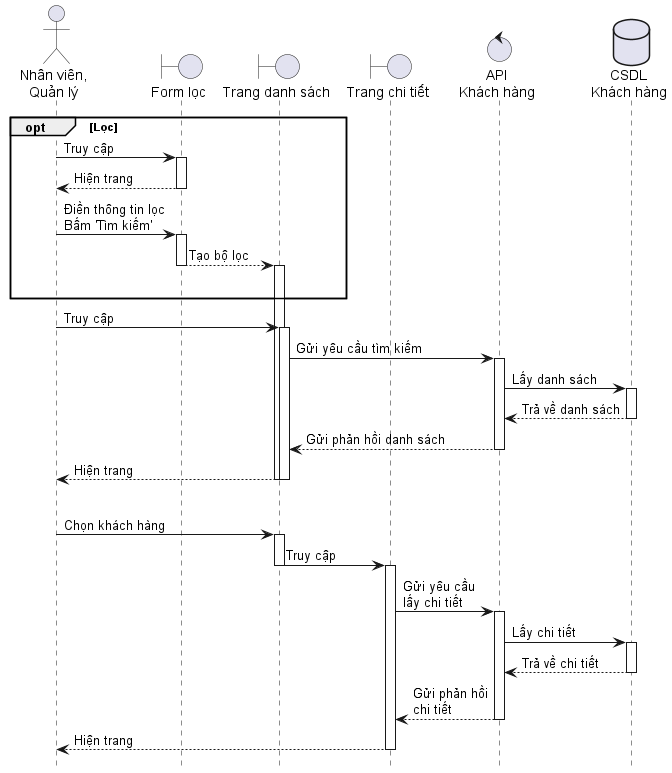
\includegraphics[width=0.7\textwidth]{Hinhve/sequences/ClientFilter.png}
    \caption{Biểu đồ tuần tự use case Lọc và xem khách hàng}
    \label{figure:sd-client-filter}
\end{figure}
\break


\subsection{Đặc tả use case Quản lý khách hàng}
\label{section:uc-client-manage}
Bảng \ref{table:uc-client-manage} mô tả chi tiết use case Quản lý khách hàng. Hình \ref{figure:sd-client-manage} mô tả biểu đồ tuần tự của use case này.
\begin{figure}[H]
    \centering
    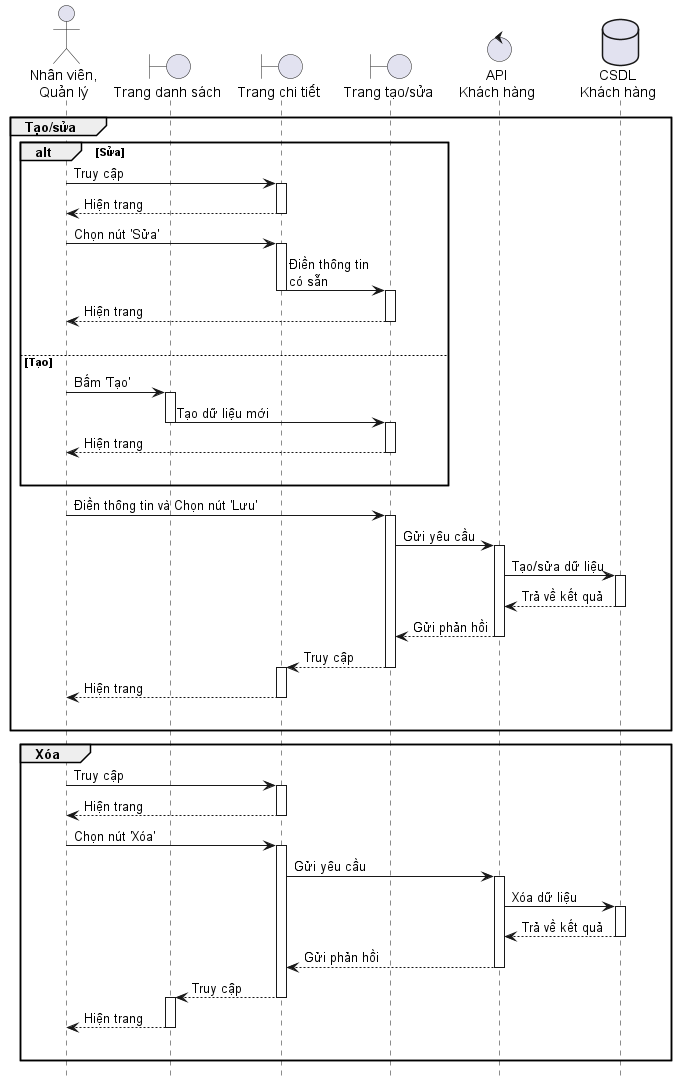
\includegraphics[width=0.9\textwidth]{Hinhve/sequences/ClientManage.png}
    \caption{Biểu đồ tuần tự use case Quản lý khách hàng}
    \label{figure:sd-client-manage}
\end{figure}
\break

\begin{table}[H]
    \begin{tabular}{|l|c|l|l|}
        \hline
        \textbf{Mã Use case}                    & \multicolumn{3}{l|}{UC61}                                                                                                                                    \\ \hline
        \textbf{Tên Use case}                   & \multicolumn{3}{l|}{Quản lý khách hàng}                                                                                                                      \\ \hline
        \textbf{Tác nhân}                       & \multicolumn{3}{l|}{Nhân viên, Quản lý}                                                                                                                      \\ \hline
        \textbf{Mô tả}                          & \multicolumn{3}{l|}{Người dùng muốn thêm, sửa, xóa khách hàng}                                                                                               \\ \hline
        \textbf{Tiền điều kiện}                 & \multicolumn{3}{l|}{Người dùng là Nhân viên hoặc Quản lý}                                                                                                    \\ \hline
        \multirow{9}{*}{\textbf{Luồng sự kiện}} & \multicolumn{1}{c|}{\textbf{STT}}                              & \multicolumn{1}{c|}{\textbf{Hành động}}   & \multicolumn{1}{c|}{\textbf{Hệ thống phản hồi}} \\ \cline{2-4}
                                                & \multirow{3}{*}{\textbf{1}}                                    & Chọn nút tạo mới ' + '                    & Hiện form tạo                                   \\ \cline{3-4}
                                                &                                                                & Điền thông tin                            &                                                 \\
                                                &                                                                & Chọn nút 'Lưu'                            & Hiện màn danh sách                              \\ \cline{2-4}
                                                & \multirow{4}{*}{\textbf{2}}                                    & Chọn khách hàng                           & Hiện màn thông tin                              \\ \cline{3-4}
                                                &                                                                & Chọn nút ' \vdots{} ' $\rightarrow$ 'Sửa' & Hiện form sửa                                   \\ \cline{3-4}
                                                &                                                                & Điền thông tin                            &                                                 \\
                                                &                                                                & Chọn nút 'Lưu'                            & Hiện màn thông tin                              \\ \cline{2-4}
                                                & \multirow{1}{*}{\textbf{3}}                                    & Chọn nút ' \vdots{} ' $\rightarrow$ 'Xóa' & Hiện màn danh sách                              \\ \hline
        \textbf{Hậu điều kiện}                  & \multicolumn{3}{l|}{Thêm, sửa, xóa thông tin thành công}                                                                                                     \\ \hline
    \end{tabular}
    \caption{Đặc tả use case Quản lý khách hàng}
    \label{table:uc-client-manage}
\end{table}


\subsection{Đặc tả use case Tìm kiếm khách hàng}
\label{section:uc-client-search}
Bảng \ref{table:uc-client-search} mô tả chi tiết use case Tìm kiếm khách hàng. Hình \ref{figure:sd-client-search} mô tả biểu đồ tuần tự của use case này.
\begin{table}[H]
    \begin{tabular}{|l|c|l|l|}
        \hline
        \textbf{Mã Use case}                    & \multicolumn{3}{l|}{UC62}                                                                                                                               \\ \hline
        \textbf{Tên Use case}                   & \multicolumn{3}{l|}{Tìm kiếm khách hàng}                                                                                                                \\ \hline
        \textbf{Tác nhân}                       & \multicolumn{3}{l|}{Nhân viên, Quản lý}                                                                                                                 \\ \hline
        \multirow{2}{*}{\textbf{Mô tả} }        & \multicolumn{3}{l|}{Người dùng muốn tìm kiếm khách hàng}                                                                                                \\
                                                & \multicolumn{3}{l|}{để thêm vào đơn từ}                                                                                                                 \\ \hline
        \textbf{Tiền điều kiện}                 & \multicolumn{3}{l|}{Người dùng là Nhân viên hoặc Quản lý}                                                                                               \\ \hline
        \multirow{4}{*}{\textbf{Luồng sự kiện}} & \multicolumn{1}{c|}{\textbf{STT}}                           & \multicolumn{1}{c|}{\textbf{Hành động}} & \multicolumn{1}{c|}{\textbf{Hệ thống phản hồi}} \\ \cline{2-4}
                                                & \multirow{3}{*}{\textbf{1}}                                 & Điền tên hoặc số điện thoại             & Hiện danh sách chuỗi                            \\
                                                &                                                             & khách hàng                              & khách hàng                                      \\
                                                &                                                             & Chọn ô thông tin sản phẩm               & Quay về màn đơn từ                              \\ \hline
        \textbf{Hậu điều kiện}                  & \multicolumn{3}{l|}{Tìm kiếm và thêm khách hàng vào đơn từ}                                                                                             \\ \hline
    \end{tabular}
    \caption{Đặc tả use case Tìm kiếm khách hàng}
    \label{table:uc-client-search}
\end{table}
\break

\begin{figure}[H]
    \centering
    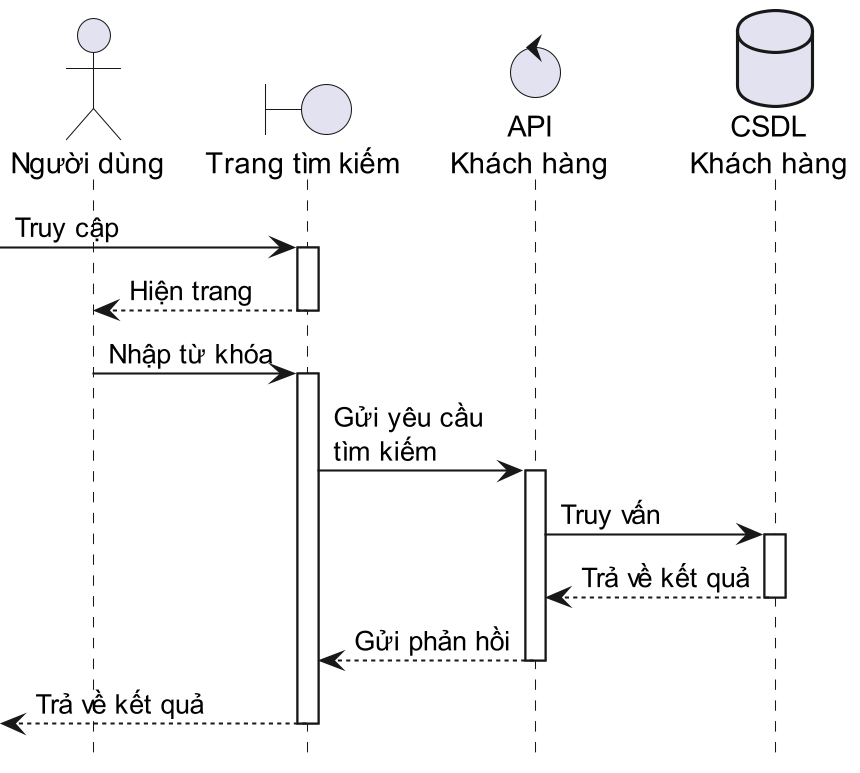
\includegraphics[width=0.6\textwidth]{Hinhve/sequences/ClientSearch.png}
    \caption{Biểu đồ tuần tự use case Tìm kiếm khách hàng}
    \label{figure:sd-client-search}
\end{figure}


\subsection{Đặc tả use case Quản lý người dùng}
\label{section:uc-user-manage}
Bảng \ref{table:uc-user-manage} mô tả chi tiết use case Quản lý người dùng. Hình \ref{figure:sd-user-manage1} và \ref{figure:sd-user-manage2} mô tả biểu đồ tuần tự của use case này.
\begin{table}[H]
    \begin{tabular}{|l|c|l|l|}
        \hline
        \textbf{Mã Use case}                     & \multicolumn{3}{l|}{UC70}                                                                                                                                                  \\ \hline
        \textbf{Tên Use case}                    & \multicolumn{3}{l|}{Quản lý người dùng}                                                                                                                                    \\ \hline
        \textbf{Tác nhân}                        & \multicolumn{3}{l|}{Quản trị viên}                                                                                                                                         \\ \hline
        \multirow{2}{*}{\textbf{Mô tả} }         & \multicolumn{3}{l|}{Người dùng muốn xem chi tiết, thêm, sửa,}                                                                                                              \\
                                                 & \multicolumn{3}{l|}{thay đổi mật khẩu, xóa người dùng}                                                                                                                     \\ \hline
        \textbf{Tiền điều kiện}                  & \multicolumn{3}{l|}{Người dùng là Quản trị viên}                                                                                                                           \\ \hline
        \multirow{9}{*}{\textbf{Luồng sự kiện}}  & \multicolumn{1}{c|}{\textbf{STT}}                                            & \multicolumn{1}{c|}{\textbf{Hành động}}   & \multicolumn{1}{c|}{\textbf{Hệ thống phản hồi}} \\ \cline{2-4}
                                                 & \multirow{3}{*}{\textbf{1}}                                                  & Chọn nút tạo mới ' + '                    & Hiện form tạo                                   \\ \cline{3-4}
                                                 &                                                                              & Điền thông tin                            &                                                 \\
                                                 &                                                                              & Chọn nút 'Lưu'                            & Hiện màn danh sách                              \\ \cline{2-4}
                                                 & \multirow{2}{*}{\textbf{2}}                                                  & Chọn ô người dùng                         & Hiện màn thông tin                              \\ \cline{3-4}
                                                 &                                                                              & Chọn nút 'Reset mật khẩu'                 & Thông báo mật khẩu mới                          \\ \cline{2-4}
                                                 & \multirow{3}{*}{\textbf{3}}                                                  & Chọn nút ' \vdots{} ' $\rightarrow$ 'Sửa' & Hiện form sửa                                   \\ \cline{3-4}
                                                 &                                                                              & Điền thông tin                            &                                                 \\
                                                 &                                                                              & Chọn nút 'Lưu'                            & Hiện màn thông tin                              \\ \cline{2-4}
                                                 & \multirow{1}{*}{\textbf{4}}                                                  & Chọn nút ' \vdots{} ' $\rightarrow$ 'Xóa' & Hiện màn danh sách                              \\ \hline
        \multirow{4}{*}{\textbf{Luồng ngoại lệ}} & \multicolumn{1}{c|}{\textbf{STT}}                                            & \multicolumn{1}{c|}{\textbf{Hành động}}   & \multicolumn{1}{c|}{\textbf{Hệ thống phản hồi}} \\ \cline{2-4}
                                                 & \multirow{3}{*}{\textbf{1}}                                                  & Chọn nút tạo mới ' + '                    & Hiện form tạo                                   \\ \cline{3-4}
                                                 &                                                                              & Điền thông tin                            & Thông báo tên đăng                              \\
                                                 &                                                                              & Chọn nút 'Lưu'                            & nhập đã tồn tại                                 \\ \hline
        \textbf{Hậu điều kiện}                   & \multicolumn{3}{l|}{Thêm, sửa, thay đổi mật khẩu, xóa người dùng thành công}                                                                                               \\ \hline
    \end{tabular}
    \caption{Đặc tả use case Quản lý người dùng}
    \label{table:uc-user-manage}
\end{table}
\break

\begin{figure}[H]
    \centering
    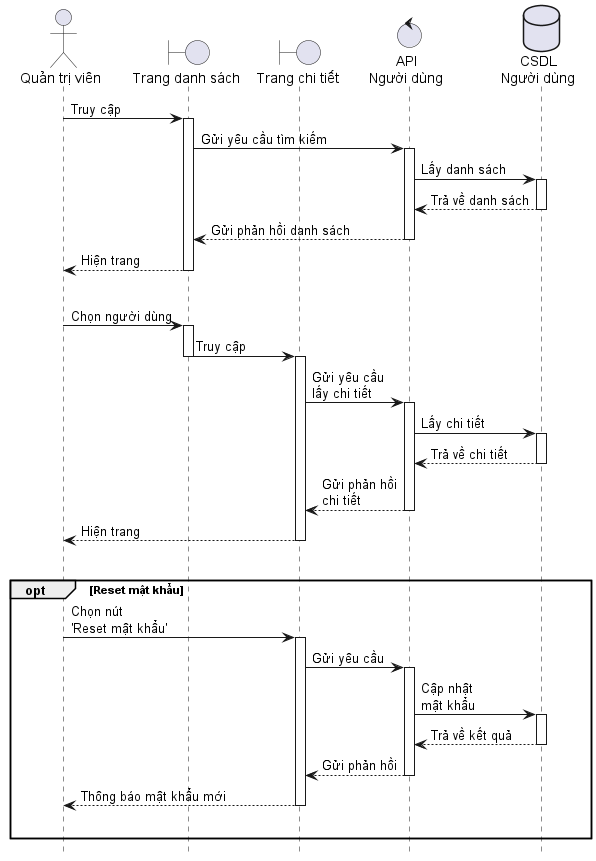
\includegraphics[width=1\textwidth]{Hinhve/sequences/UserManage1.png}
    \caption{Biểu đồ tuần tự use case Quản lý người dùng (phần 1)}
    \label{figure:sd-user-manage1}
\end{figure}
\break

\begin{figure}[H]
    \centering
    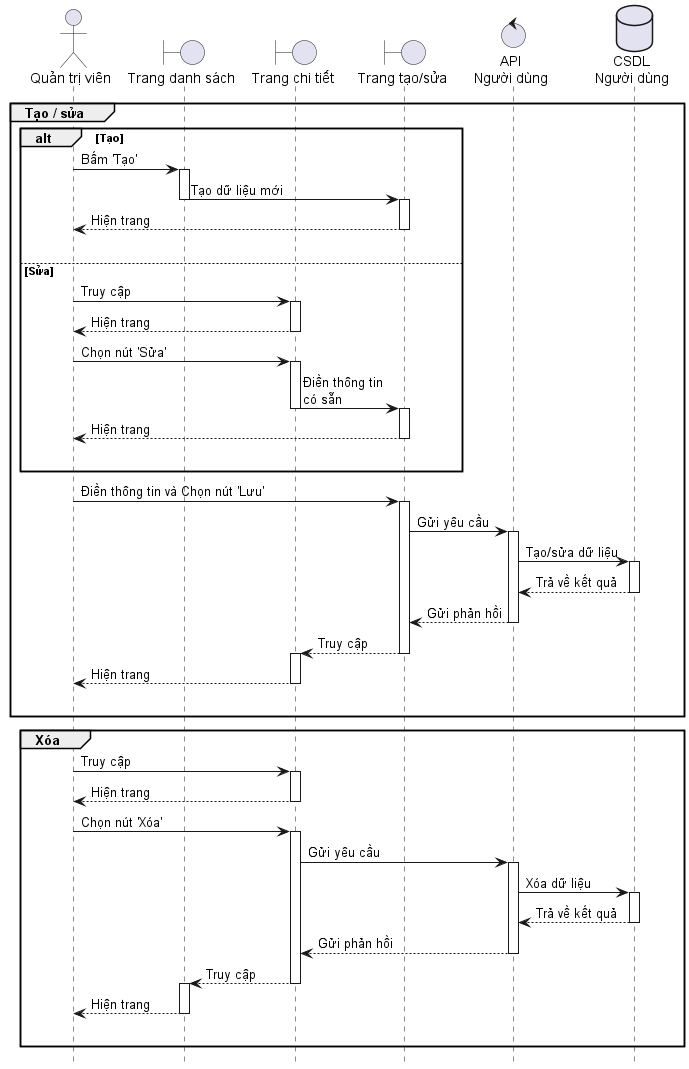
\includegraphics[width=1\textwidth]{Hinhve/sequences/UserManage2.png}
    \caption{Biểu đồ tuần tự use case Quản lý người dùng (phần 2)}
    \label{figure:sd-user-manage2}
\end{figure}
\break


\subsection{Đặc tả use case Quản lý thông tin cá nhân}
\label{section:uc-user-memanage}
Bảng \ref{table:uc-user-memanage} mô tả chi tiết use case Quản lý thông tin cá nhân. Hình \ref{figure:sd-user-memanage} mô tả biểu đồ tuần tự của use case này.
\begin{table}[H]
    \begin{tabular}{|l|c|l|l|}
        \hline
        \textbf{Mã Use case}                    & \multicolumn{3}{l|}{UC71}                                                                                                                                      \\ \hline
        \textbf{Tên Use case}                   & \multicolumn{3}{l|}{Quản lý thông tin cá nhân}                                                                                                                 \\ \hline
        \textbf{Tác nhân}                       & \multicolumn{3}{l|}{Quản trị viên, Quản lý, Nhân viên}                                                                                                         \\ \hline
        \multirow{2}{*}{\textbf{Mô tả} }        & \multicolumn{3}{l|}{Người dùng muốn xem chi tiết, sửa thông tin}                                                                                               \\
                                                & \multicolumn{3}{l|}{người dùng cá nhân}                                                                                                                        \\ \hline
        \textbf{Tiền điều kiện}                 & \multicolumn{3}{l|}{Đã đăng nhập hệ thống}                                                                                                                     \\ \hline
        \multirow{5}{*}{\textbf{Luồng sự kiện}} & \multicolumn{1}{c|}{\textbf{STT}}                                & \multicolumn{1}{c|}{\textbf{Hành động}}   & \multicolumn{1}{c|}{\textbf{Hệ thống phản hồi}} \\ \cline{2-4}
                                                & \multirow{1}{*}{\textbf{1}}                                      & Chọn thanh thông tin cá nhân              & Hiện màn thông tin                              \\ \cline{2-4}
                                                & \multirow{3}{*}{\textbf{2}}                                      & Chọn nút ' \vdots{} ' $\rightarrow$ 'Sửa' & Hiện form sửa                                   \\ \cline{3-4}
                                                &                                                                  & Điền thông tin                            &                                                 \\
                                                &                                                                  & Chọn nút 'Lưu'                            & Hiện màn thông tin                              \\ \hline
        \textbf{Hậu điều kiện}                  & \multicolumn{3}{l|}{Xem chi tiết, sửa thông tin thành công}                                                                                                    \\ \hline
    \end{tabular}
    \caption{Đặc tả use case Quản lý thông tin cá nhân}
    \label{table:uc-user-memanage}
\end{table}
\begin{figure}[H]
    \centering
    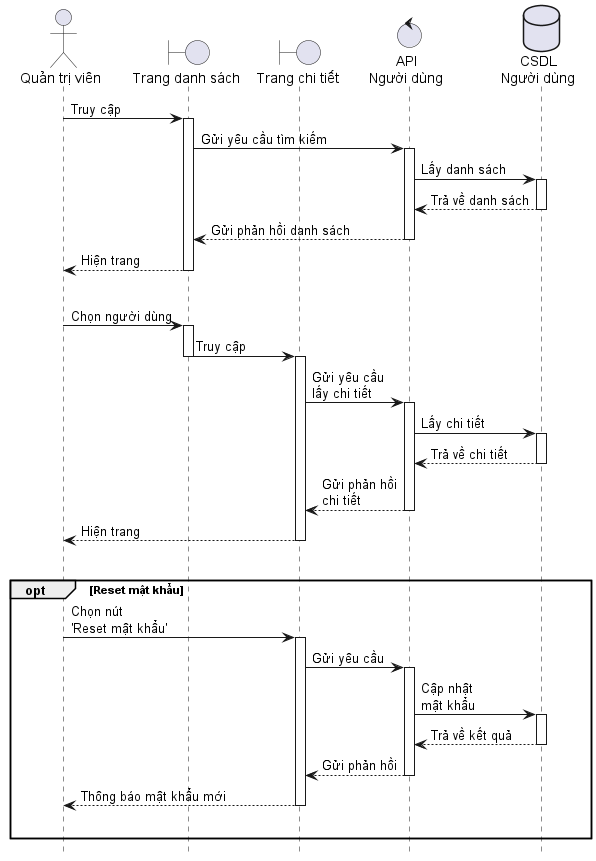
\includegraphics[width=0.6\textwidth]{Hinhve/sequences/UserMeManage.png}
    \caption{Biểu đồ tuần tự use case Quản lý thông tin cá nhân}
    \label{figure:sd-user-memanage}
\end{figure}
\break
% END OF SECTION


% START OF SECTION
\section{Yêu cầu phi chức năng}
\label{section:ycpcn}
% Trong phần này, sinh viên đưa ra các yêu cầu khác nếu có, bao gồm các yêu cầu phi chức năng như hiệu năng, độ tin cậy, tính dễ dùng, tính dễ bảo trì, hoặc các yêu cầu về mặt kỹ thuật như về CSDL, công nghệ sử dụng, v.v.
Ngoài các bộ usecase đã được trình bày ở trên, hệ thống còn có các yêu cầu phi chức năng như sau để đạt được mục tiêu của dự án:
\begin{itemize}
    \item Hệ thống backend phải có thể chạy trên các hệ điều hành Windows, Linux.
    \item Ứng dụng người dùng phải chạy được trên các thiết bị di động Android, iOS.
    \item Hệ thống phải có khả năng chịu tải tối thiểu 100 request trên 1 giây.
    \item Lưu lượng sử dụng mạng nên được tối giản và tối ưu nhất đề phòng sự cố nghẽn mạng.
    \item Khả năng bảo trì và hồi phục hệ thống trong vòng 1 giờ.
    \item Dự án có một bộ codebase dễ dàng mở rộng và bảo trì.
    \item Dễ cài đặt và có hướng dẫn tường minh cho người quản trị.
    \item Tính bảo mật cao, hệ thống phải có khả năng chống lại các cuộc tấn công từ bên ngoài.
\end{itemize}


%  END OF SECTION
\end{document}